%!TEX root = ../xesphVI.tex
\chapter{光学成像}

\section{傍轴光成像}

\subsection{物与像}
\begin{wrapfigure}[13]{o}[-10pt]{6cm}
\centering
\vspace{-1cm}
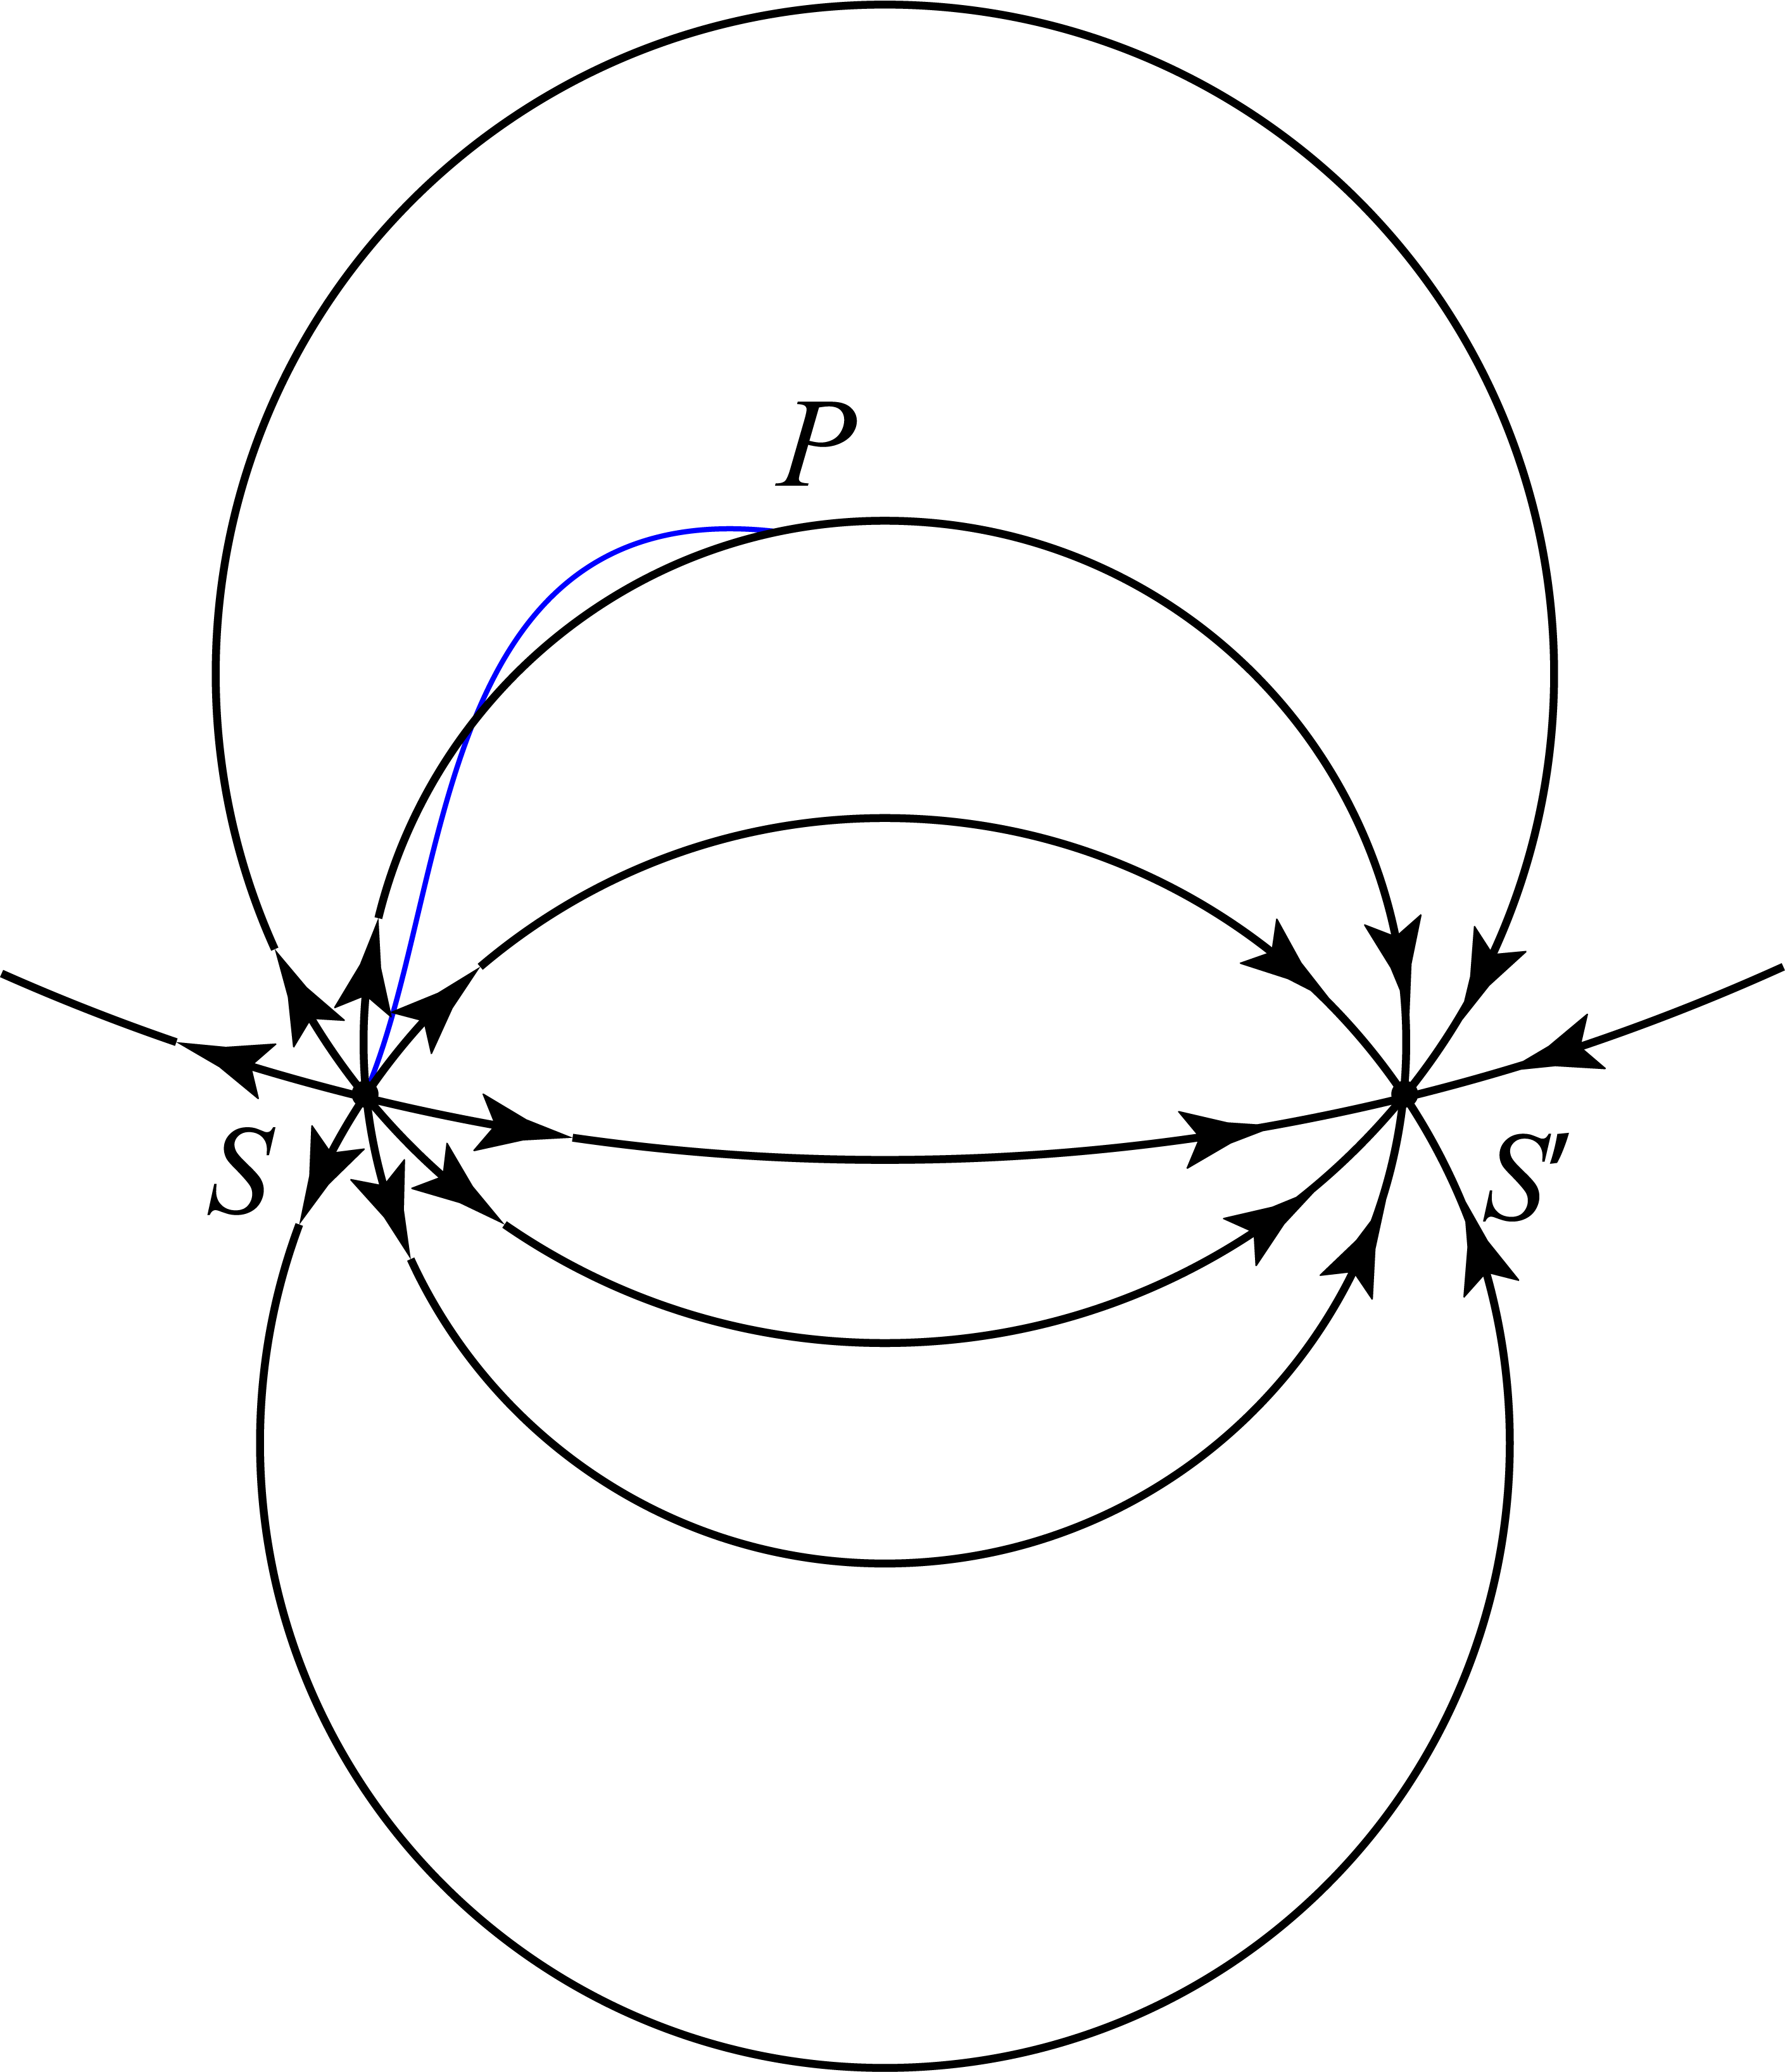
\includegraphics[width=6cm]{image/5-7-1.png}
\caption{物与像}
\end{wrapfigure}
成像不是一个平凡的过程.\,延续上一章我们对变折射率问题的讨论,\,现在我们引入所谓\emph{物}(object)的概念,\,它指的是一个点光源\(S\),\,它能够向各种不同的方向发射光线,\,每一个既定的方向则可以根据光线方程求解之后的光线传播.\,这样它所发出的光场构成了物的光场.\,而传播过程中到达的任何一点\(P\),\,满足\(S\)与\(P\)间的真实光线有且只有一条.\,它恰好由费马原理确定.\,但传播过程中可能发生一种奇异的现象,\,就是在空间中另一点\(S'\)处成了\emph{像}(image).\,从光线角度看,\,便是:

\begin{quote}
一定范围内,\,物发出的每一条光线都经过像.
\end{quote}

而根据费马原理,\,真实光线旁边的微扰光线光程对此光线的一阶变分为零,\,但此时有一大组真实光线,\,彼此之间可以连续的过渡,\,我们必然得出:

\begin{quote}
物与像之间的所有真实光线,\,其光程都是相等的.
\end{quote}

以上就是物像之间的\emph{等光程原理}(the principle of equal path length).\,它实际上也是作为了能否成像,\,成像在何处的判据.\,这一个结论也可以依靠干涉理论,\,或者更普遍的,\,光场概率幅的路径积分理论来理解:\,如果两点间光程沿某种路径不是取得极值,\,那么这种情形将会由于存在很多其他类似的路径,\,使得最后在终点处贡献的概率幅相干相消.\,仅仅是在光程取得极值的路径将对最后终点处的概率幅有主要贡献.\,但在物像点间如果存在大量路径其光程完全不变,\,最后像点的概率幅将会非常地大,\,这也就是成像的过程了.

\begin{wrapfigure}[13]{o}[-10pt]{7cm}
\centering
\vspace{0cm}
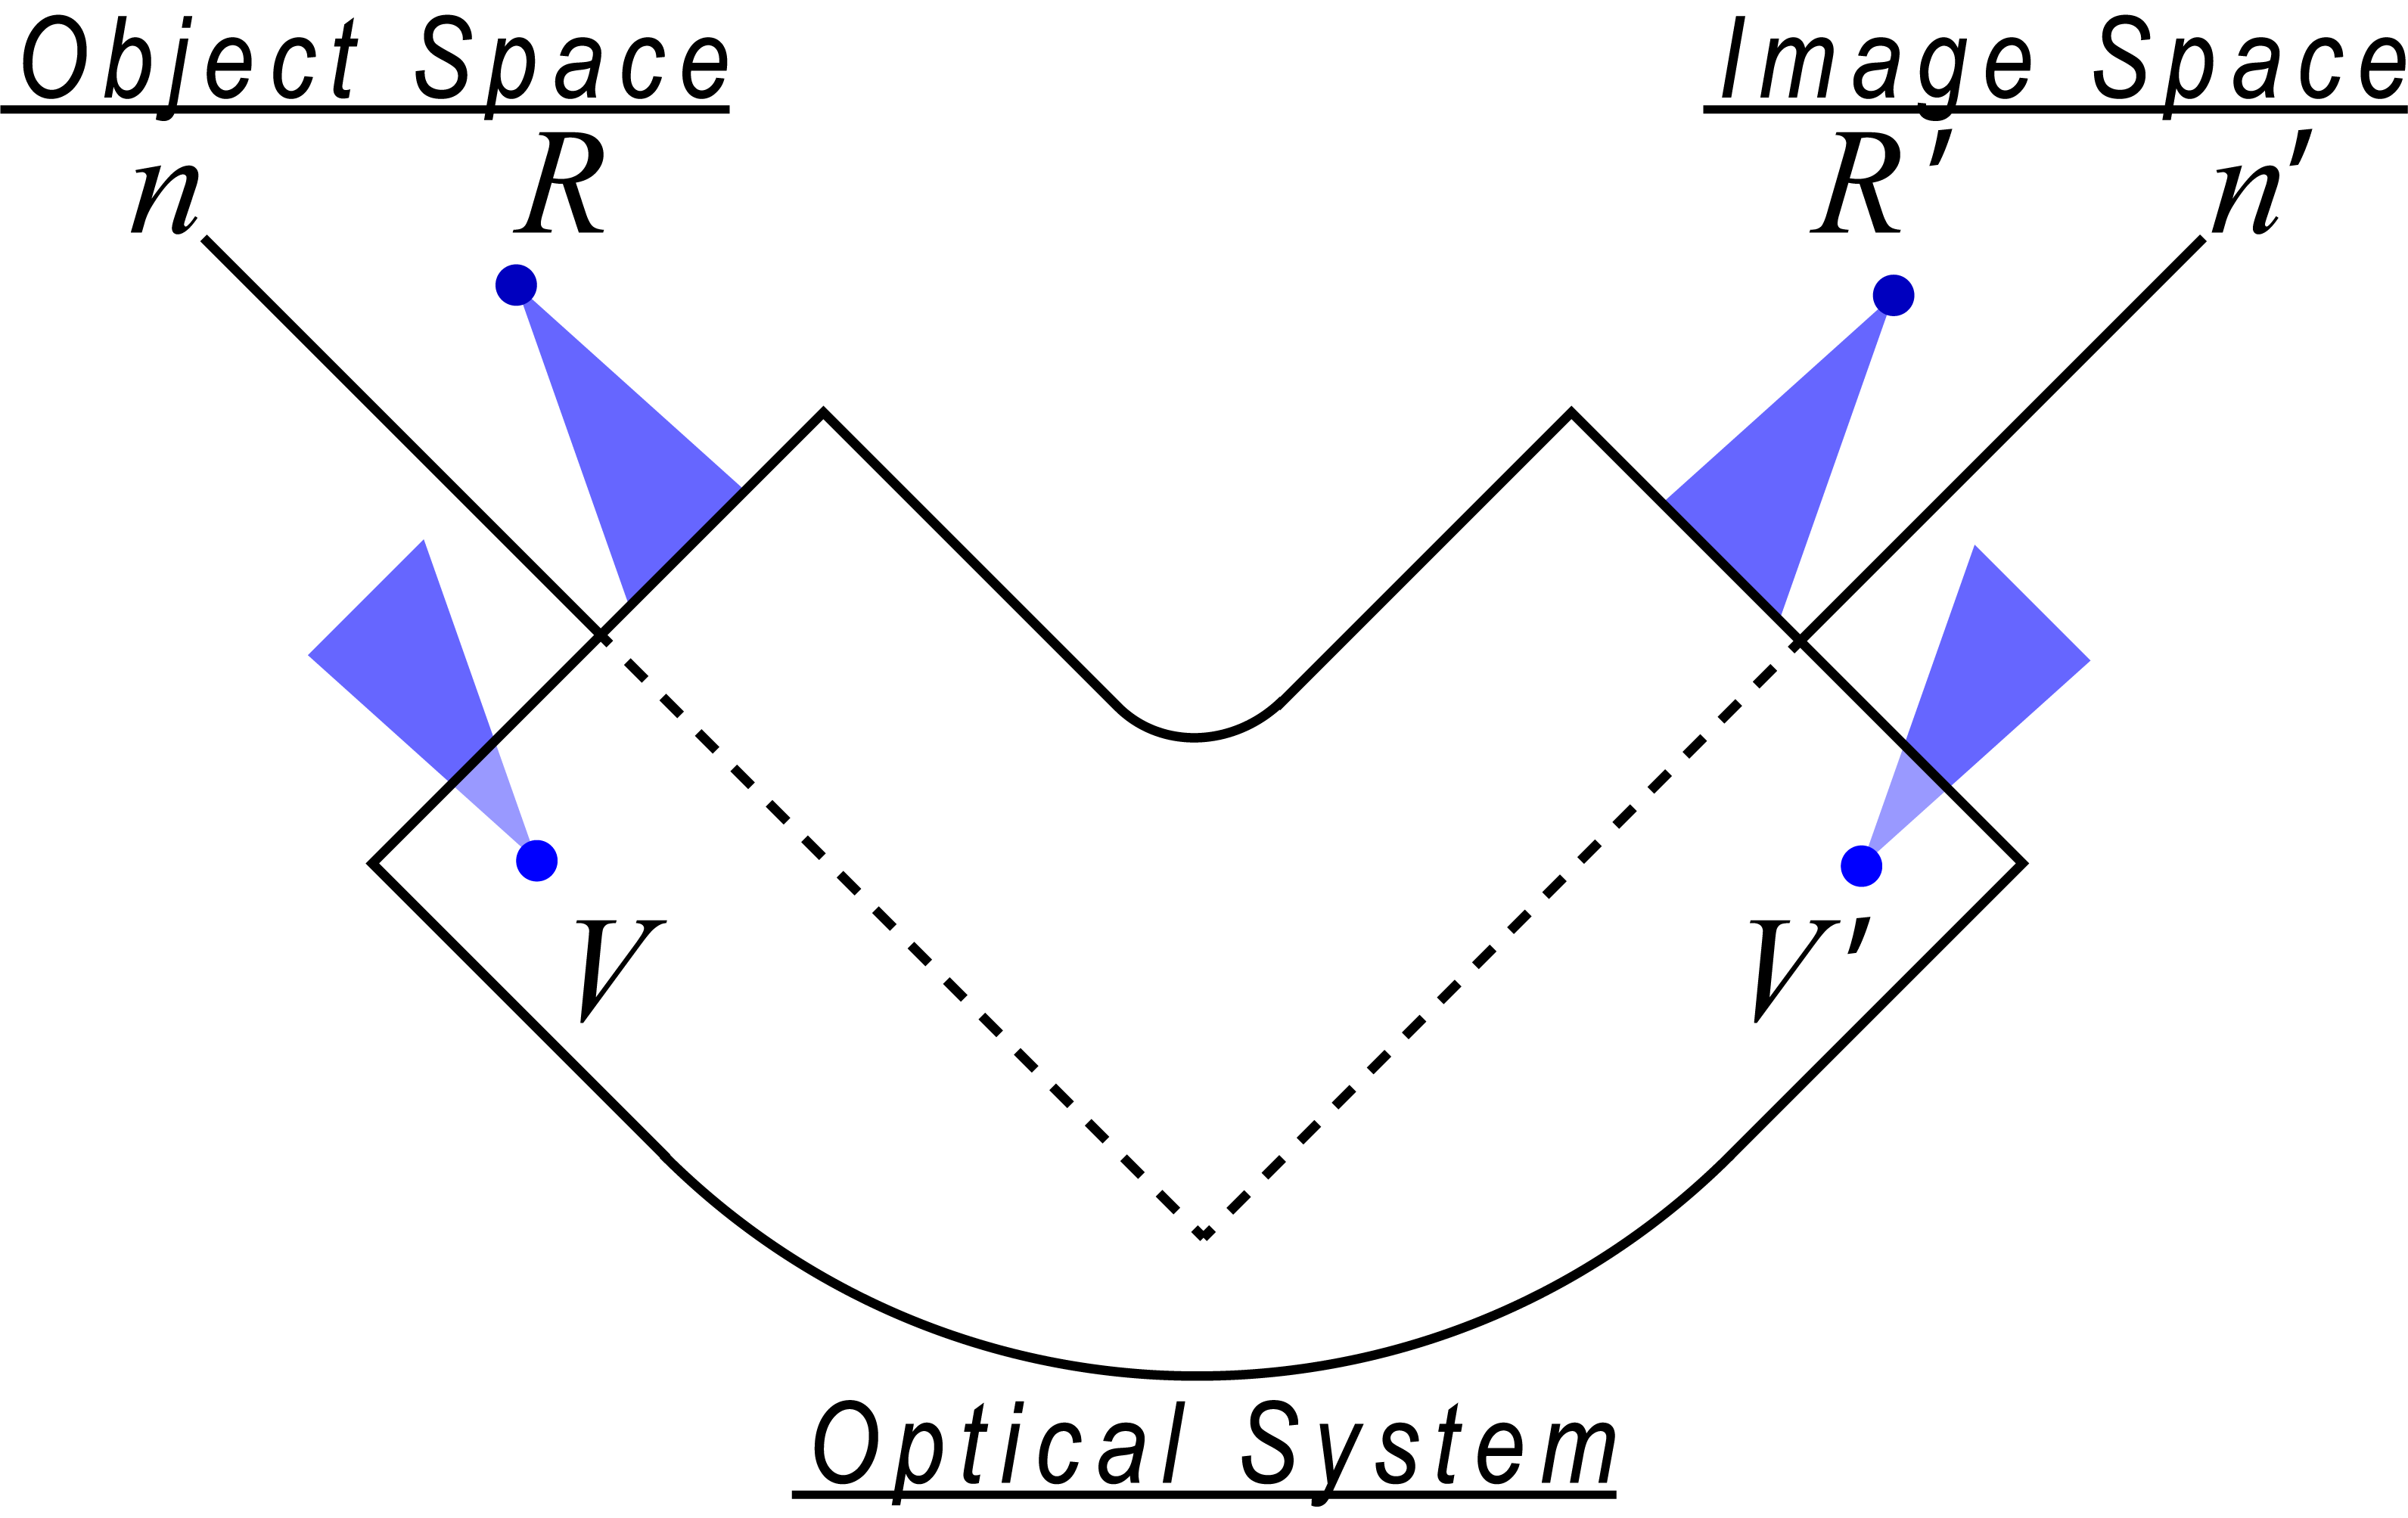
\includegraphics[width=7cm]{image/5-7-2.png}
\caption{实与虚}
\end{wrapfigure}
以上描述的实际上只是几何光学中的实物与实像的概念.\,在一般的光学系统中,\,光路都是傍轴的.\,即满足\emph{傍轴条件}(paraxial condition):\,有一条中心光线作为\emph{主光轴}(optical axis)参考.\,\emph{光具组}(optical system)把光路分为\emph{物方}(object space)与\emph{像方}(image space).\,两个空间一般都是均匀折射率空间,\,故一般考虑\emph{光锥}(pencil)型光束的传播(就是球面波).\,注意两个空间有可能重合(反射情况).\,这样的光束偏离主光轴的角度满足:
\[\theta\ll 1\]

或者表述为
\[\frac{z}{l}\ll 1\]

其中\(z\)是光路的特征偏离主光轴的距离.\,而\(l\)是光路沿主光轴传播的特征长度.\,如果进入光具组时光束呈现\emph{发散}(diverging)态,\,则说明进入光具组前已有物,\,尽管这一个物有可能也不在真实空间中(如前一次经过光学组后成虚像作为这次的实物),\,也把这样的物称为\emph{实物}(real object).\,它一定位于物方.\,而相反的情况是进入光具组时为\emph{会聚}(converging)光的情况,\,那么物就不可能在物方找到了,\,它位于光具入射面的另一侧(不一定是像方),\,这样的物称为\emph{虚物}(virtual object).\,同理,\,对于像,\,出射光会聚的像位于像方,\,是\emph{实像}(real image),\,而出射光发散,\,像位于像方的另一侧,\,则是\emph{虚像}(virtual image).

\subsection{球对称成像系统与符号法则}
顾名思义,\,球对称成像系统指的是主光轴在一条直线上而整个光具组具有对主光轴的旋转对称性.\,当然实际光锥光路不一定要求关于主光轴对称.\,两种典型的基础光具是折射球面与反射球面.\,如下图所示:
\begin{figure}[H]
\centering
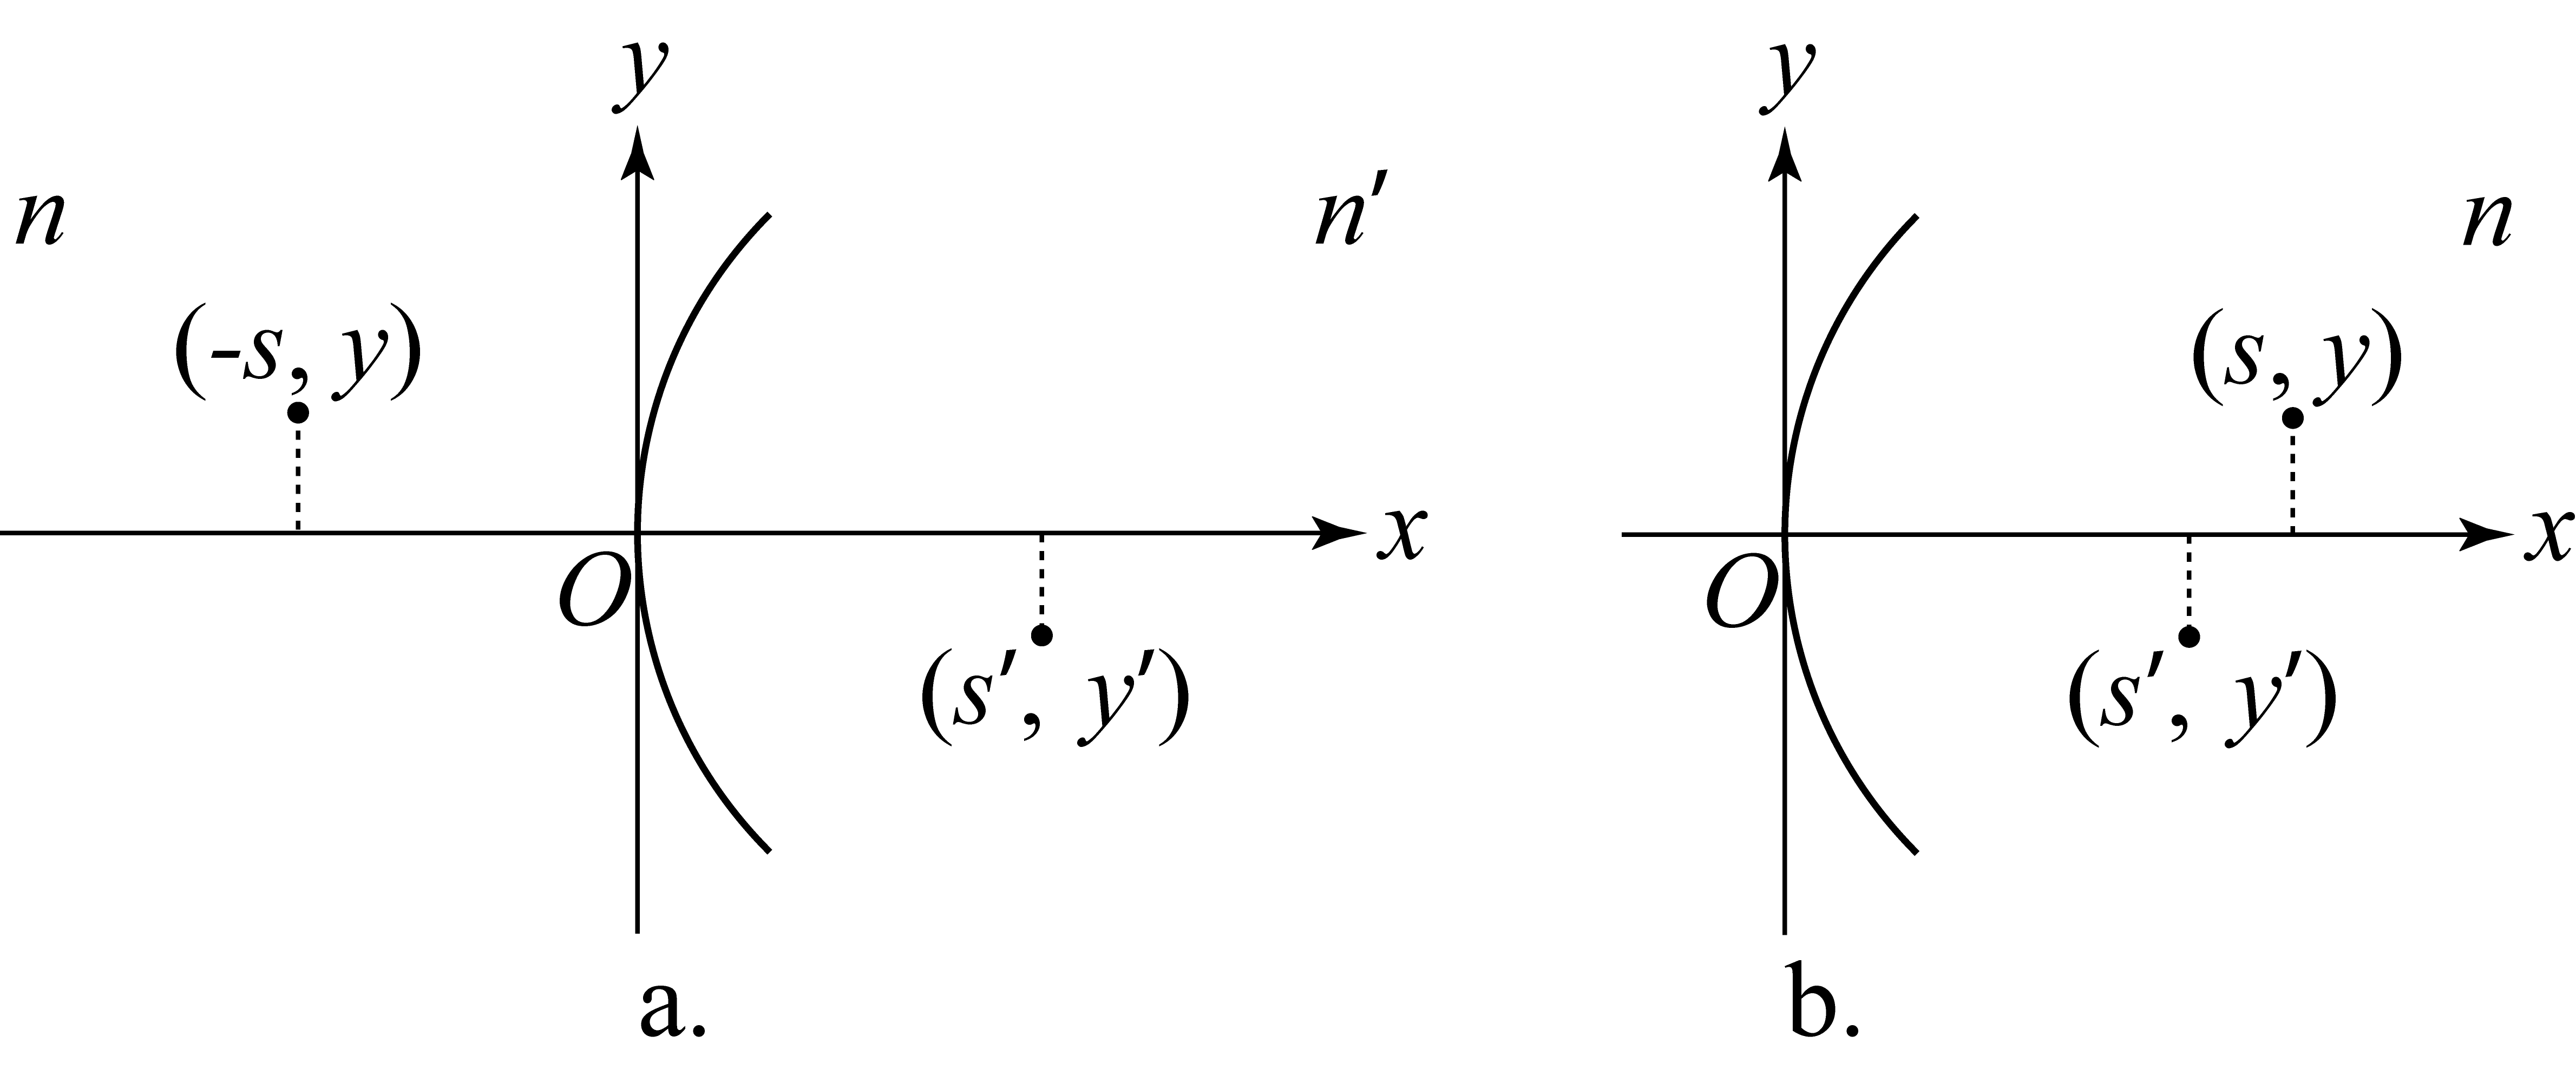
\includegraphics[width=0.9\textwidth]{image/5-7-3.png}
\caption{球面折射与球面反射}
\label{fig5-7-3}
\end{figure}

在球面折射情况\ref{fig5-7-3}下,\,我们先考虑向像方凹的,\,曲率半径为\(R\)的近似球面的傍轴折射成像(作左图).\,各量的符号设定如图,\,\(s\)为\emph{物距}(object distance),\,\(s'\)为\emph{像距}(image distance),\,\(y,\,y'\)则为物,\,像的\emph{高}(height).\,由物像的等光程性,\,应有:
\[f(X,\,Y)=n\sqrt{(X+s)^2+(Y-y)^2}+n'\sqrt{(X-s')^2+(Y-y')^2}={\rm Const.}\]

由于傍轴条件,\,上式中参量\(Y\)是理解为小量变量即可,\,而\(X\)近似为:
\[X=\frac{Y^2}{2R}\]

代入,\,小量近似,\,表示为\(Y\)的二次多项式:
\begin{align*}
f(X,\,Y)	\quad =  &\quad n\sqrt{s^2+y^2}+n'\sqrt{s'^2+y'^2}\\
			   		 &\quad -(\frac{ny}{\sqrt{s^2+y^2}}+\frac{n'y'}{\sqrt{s'^2+y'^2}})Y\\
			   		 &\quad -[\frac{n[(1+s/R)(s^2+y^2)-y^2]}{2(s^2+y^2)^{3/2}}+\frac{n'[(1-s'/R)(s'^2+y'^2)-y'^2]}{2(s'^2+y'^2)^{3/2}}]Y^2
\end{align*}

从而一次项与二次项系数都必须为零.\,由傍轴条件,\,\(s,\,s'\)是\(u,\,v\)的小量.\,从而整理得:
\[\beta=\frac{y'}{y}=-\frac{ns'}{n's}\]
\[\frac{n}{s}+\frac{n'}{s'}=\frac{n'-n}{R}\]

上式给出了成像的\emph{横向放大率}(transverse magnification)与\emph{物像距关系}(object-image distance relation),\,抽象地看,\,在傍轴加二阶近似意义下物方空间每一点都能成像.\,而给定任意物距处的像距与横向放大率,\,就决定了一个光学系统傍轴成像的所有特性.\,以上成像的两个公式的特点是:\,物像距都从球面的顶点开始计算,\,这个点称为\emph{光心}(optical centre).\,这两个公式称为\emph{高斯型公式}(Gaussian formula).\,一般把第二个物像距公式右端的结果定义为\emph{光焦度}(focusing power):
\[\varPhi=\frac{n'-n}{R}\]

其单位是\emph{屈光度}(diopter),\,中文简称``度''.\,\(1{\rm D}=1{\rm m}^{-1}\).

\begin{wrapfigure}[11]{o}[-10pt]{8cm}
\centering
\vspace{0cm}
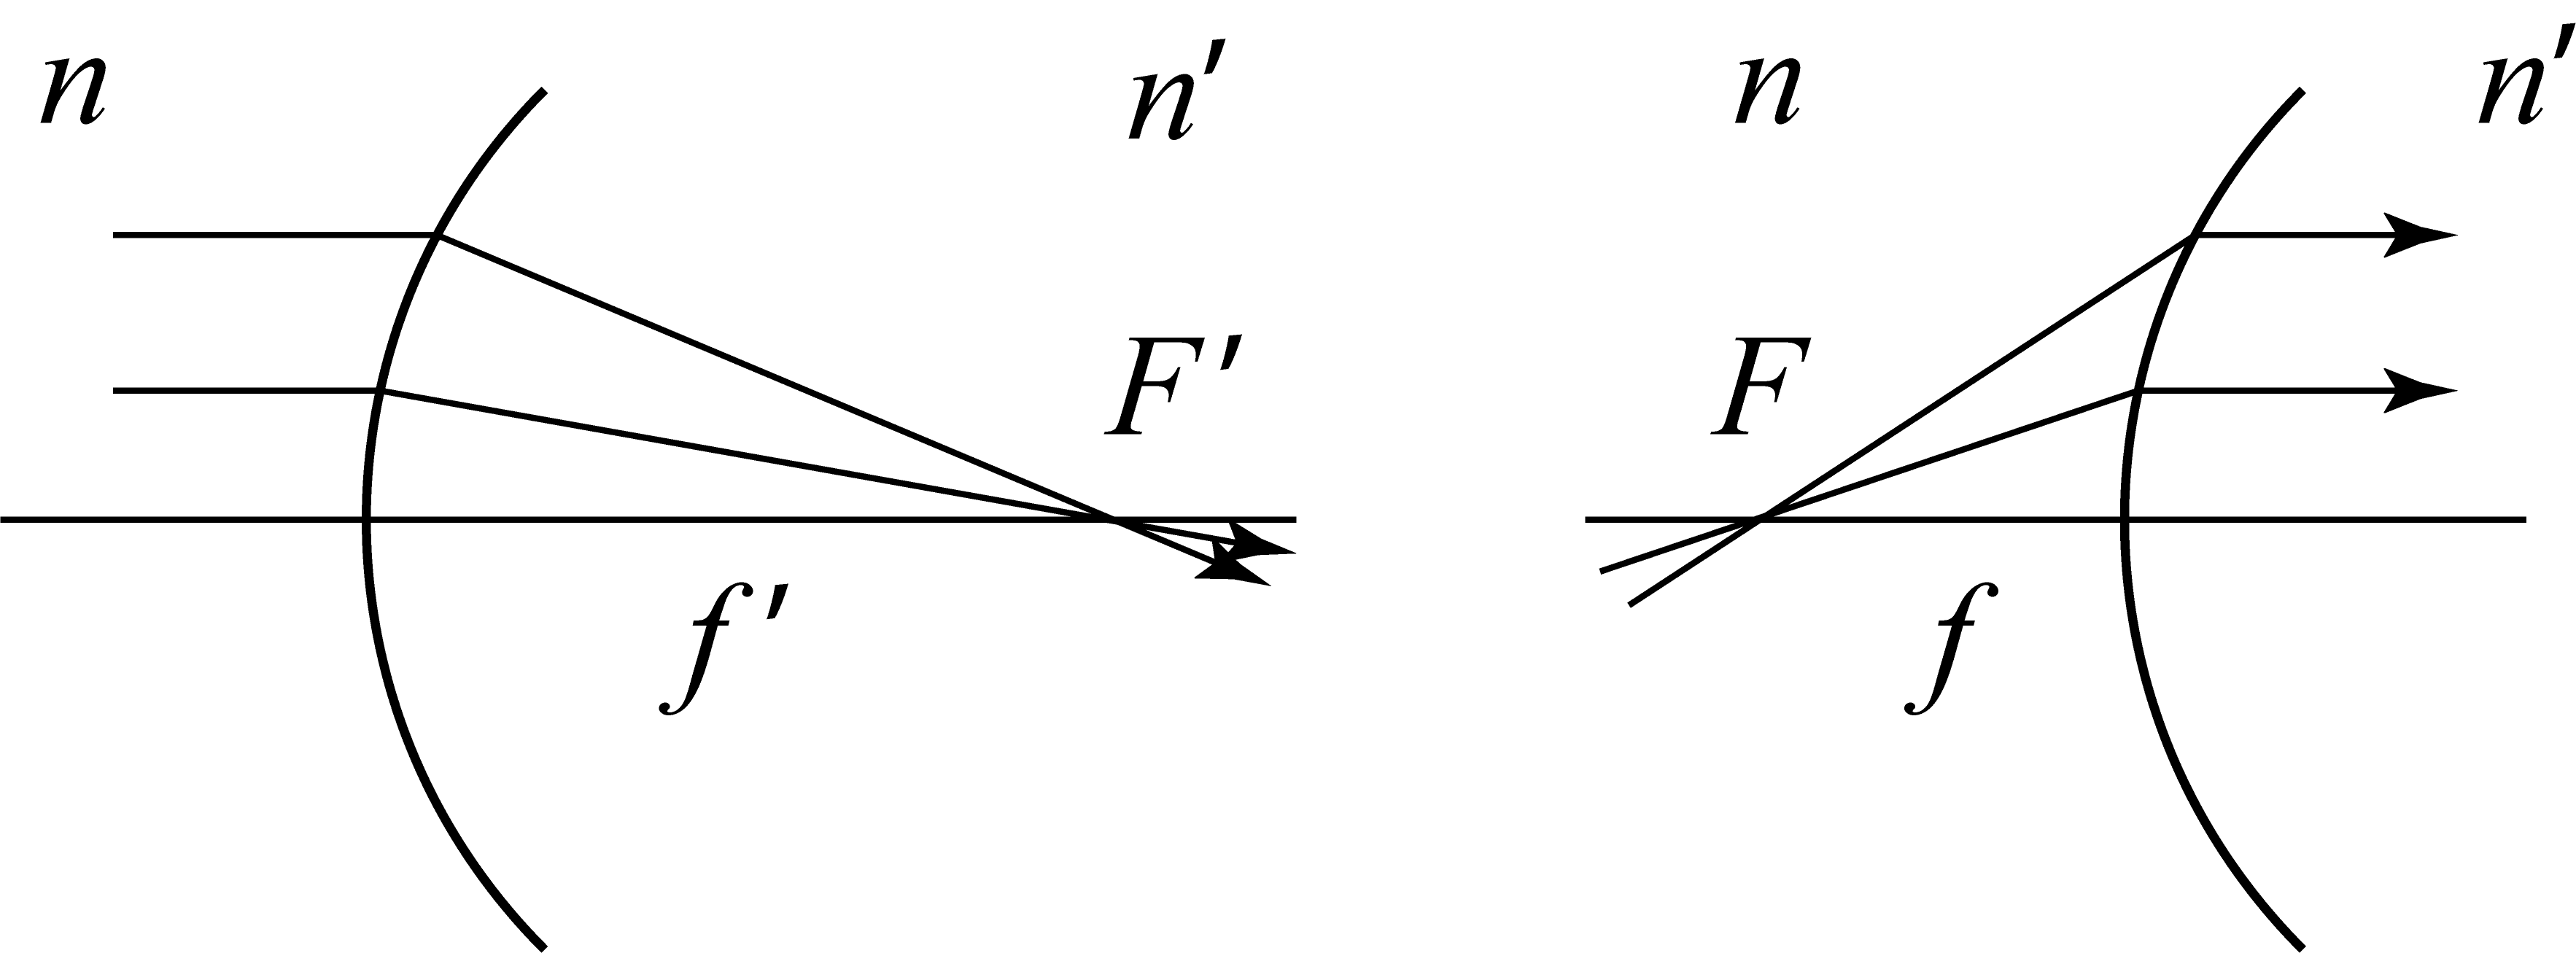
\includegraphics[width=8cm]{image/5-7-4.png}
\caption{焦点}
\end{wrapfigure}
当物距和像距取特殊值时会出现另一个趋于正负无穷,\,而对应的物像高也趋于正负无穷的情形,\,此时意味着入射,\,出射光成为了\emph{平行光}(collimated light).\,这些特殊的物像距称为\emph{焦距}(focal length),\,而对应的主光轴上的点称为\emph{焦点}(focus).\,物方焦距与像方焦距就分别为:
\[f=\frac{n}{\varPhi}=\frac{nR}{n'-n}\quad ;\quad f'=\frac{n'}{\varPhi}=\frac{n'R}{n'-n}\]

自然地有:
\[f:f'=n:n'\]

通过引入两个焦距我们可以把成像公式写作:
\[\frac{f}{s}+\frac{f'}{s'}=1\quad ;\quad \beta=-\frac{fs'}{f's}\]

实际上,\,\(n,\,n'\)都不是通过这个折射成像系统可以测量的量,\,而两个长度量纲的\(f,\,f'\)代表了这个系统成像的所有特征.

为了更直观地反应物像距指尖关系的特性,\,一般把顺光传播方向,\,物到物方焦点的距离记为另一种物距\(x=s-f\),\,而像方焦点到像的距离记为另一种像距\(x'=s'-f'\).\,那么代入高斯型公式化简可得:
\[xx'=ff'\]
\[\beta=-\frac{f}{x}=-\frac{x'}{f'}\]

以上两个公式更为精简,\,称为\emph{牛顿型公式}(Newtonian formula).\,图像也更加清晰:\,物像距恰好是一个反比关系.\,而横向放大率取决于物离物方焦点有多近,\,也等效于像离像方焦点有多远.\,运用起来往往更加方便.\,仔细观察还会发现,\,仅需\(ff'\)作为整体的大小实际上已经确定了物像距的关系.\,但如果要求的是横向放大率,\,\(f,\,f'\)各自取多少就是必要的了.\,也就是说不仅需要知道两个焦点的位置,\,还得已知光心离各自有多远.

对于\ref{fig5-7-3}右图的球面反射镜,\,只需要把两个焦距定为
\[f=f'=\frac{R}{2}\]

那么高斯型公式与牛顿型公式都以完全一样的形式适用,\,只需注意此时的主光轴正方向在反射时发生了反转,\,物像距的定义会产生相应的改变,\,参照图理解即可.

当我们考虑不同的球面凹凸性,\,不同的折射率分布,\,不同的物像实虚性时显然不希望每次都重新进行推导,\,而是希望我们之前推出的结论具有普适性.\,那么实际上之前我们涉及的每个量都可以有正负(折射率除外).\,约定不同量的正负性的方法称为\emph{符号法则}(sign convention).\,本书介绍一下符号法则:

\begin{enumerate}
	\item 光具球面曲率半径:\,{\hei 出射方看,\,凹正凸负.}\,出射方也就是单次成像的像方,\,如果曲率中心位于这一侧,\,那么曲率半径计为正.\,如果在另一侧,\,计为负.
	\item 物像距,\,焦距:\,{\hei 实正虚负.}\,如果是物点发出的发散光沿主光轴正向传播到物距的零点处则为实物,\,物距计正(实物).\,如果是会聚光传播到物距零点处还未到达物点,\,则物距计负(虚物).\,同理,\,像距零点处出射会聚光可以沿主光轴传播形成像点,\,像距计正(实像).\,若像距零点处出射发散光,\,像点可以认为应在之前形成,\,像距计负(虚像).\,物方焦距是使像距趋于无穷的特殊物距.\,像方焦距是使物距趋于无穷的特殊像距.
	\item 物像高:\,{\hei 上正下负.}\,不管任何情形,\,都规定主光轴的一侧高度大于零,\,一侧小于零.\,也就是把与这个方向垂直的轴上坐标定义为高度.\,如果把主光轴理解为水平方向,\,一般上半空间物,\,像高为正,\,下半空间物像高为负.
	\item 光线的倾角:\,{\hei 增正减负.}\,有时候我们不仅关心物像点间的对应关系,\,也关心一根光线与另一根光线的对应关系.\,而实际上相互对应的光线不仅是物方入射光线与像方出射光线的关系,\,由于每一点某能成像,\,两条线上的点也是一一对应的物像点.\,此时光线的角度被定义为沿传播方向单位长度所增加的物或像高.\,如果光线从下往上传播,\,角度为正,\,从上往下则角度为负.
\end{enumerate}

我们之前推出来的,\,针对于球面折射,\,反射的公式自然是在以上符号法则下普适的.\,同样的道理也适用于之后所有情况下提出的公式.\,而且不失一般性地,\,高斯型公式与牛顿型公式其实是对任意球对称成像系统傍轴适用的.\,推广到非傍轴情形便是下一节讨论的理想成像系统.

\begin{wrapfigure}[11]{o}[-10pt]{8cm}
\centering
\vspace{0cm}
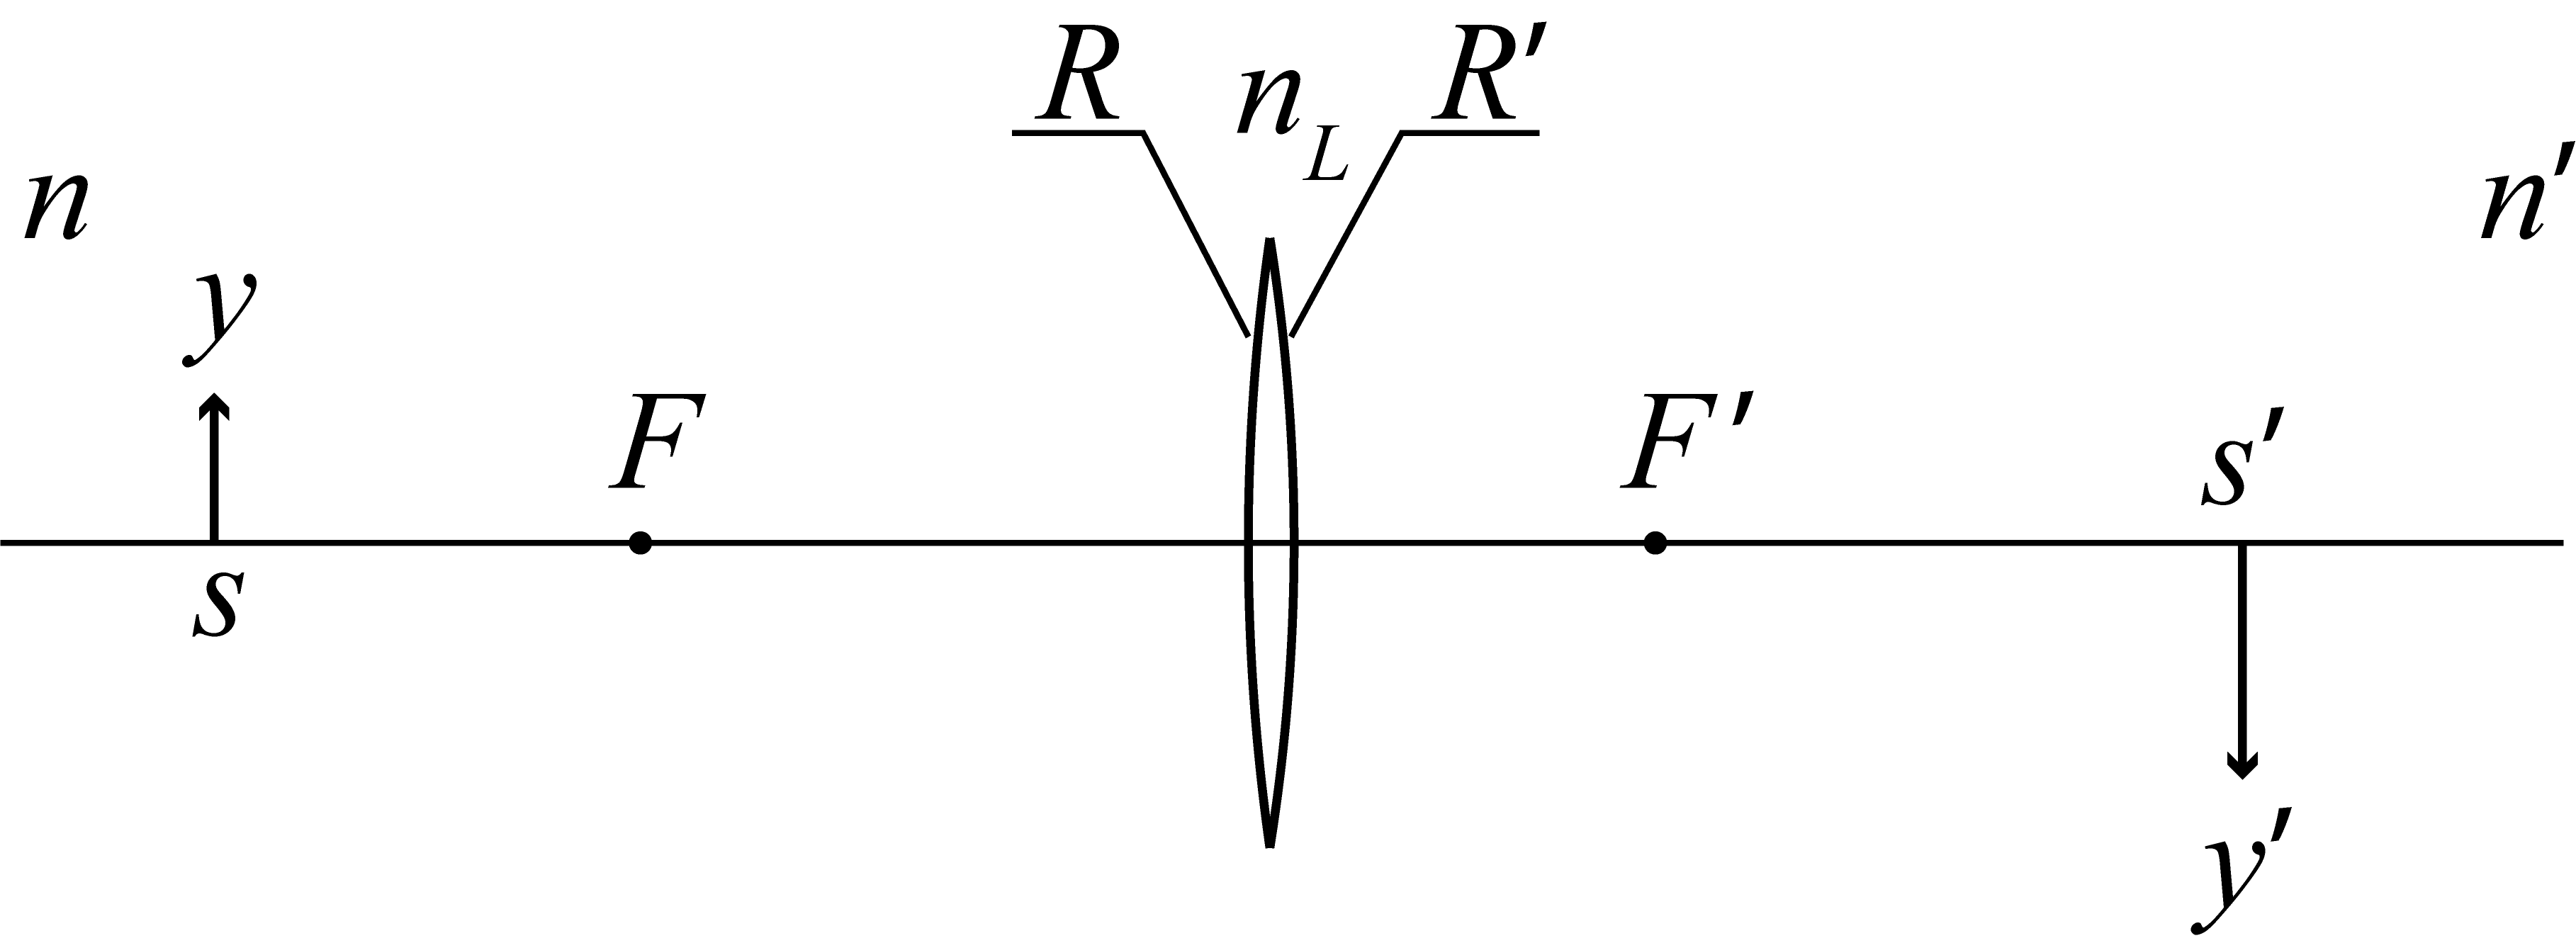
\includegraphics[width=8cm]{image/5-7-5.png}
\caption{薄透镜}
\end{wrapfigure}
我们接着讨论\emph{薄透镜}(thin lens)模型.\,这是一个两次成像的过程,\,第一次成像的像方零像距点,\,第二次成像的物方零物距点恰好重合在透镜的光心位置.\,从而有:
\[\frac{n}{s}+\frac{n_L}{s_1^\prime}=\frac{n_L-n}{R}\quad ;\quad \beta_1=-\frac{ns_1'}{n_L s}\]
\[\frac{n_L}{s_2}+\frac{n'}{s'}=\frac{n'-n_L}{-R'}\quad ;\quad \beta_2=-\frac{n_L s'}{n's_2}\]

注意在第二个公式中\(R'\)是在右表面凸是取正的曲率半径(以双凸透镜为正),\,它与我们既定的符号法则相反,\,故在照抄公式时在分母加以符号以示区别.\,再有上讨论的两个物像距参考关系:
\[s_1'+s_2=0\]

消去中间的物像距,\,得到:
\[\frac{n}{s}+\frac{n'}{s'}=\frac{n_L-n}{R}+\frac{n_L-n'}{R'}\quad ;\quad \beta=-\frac{ns'}{n's}\]

这说明把两次成像的密接的结果是光焦度的直接相加:
\[\varPhi=\varPhi_1+\varPhi_2\]

而除此以外余下公式都没有变化:
\[f=\frac{n}{\varPhi}\quad;\quad f'=\frac{n'}{\varPhi}\]
\[\frac{f}{s}+\frac{f'}{s'}=1\quad;\quad \beta=-\frac{fs'}{f's}\]

这几个规律也适用于密接的透镜组.\,任何发散和会聚光的能力直接用光焦度评价,\,密接时这些规律都直接叠加.

\subsection{光具组成像}
\begin{wrapfigure}[12]{o}[-10pt]{8cm}
\centering
\vspace{0cm}
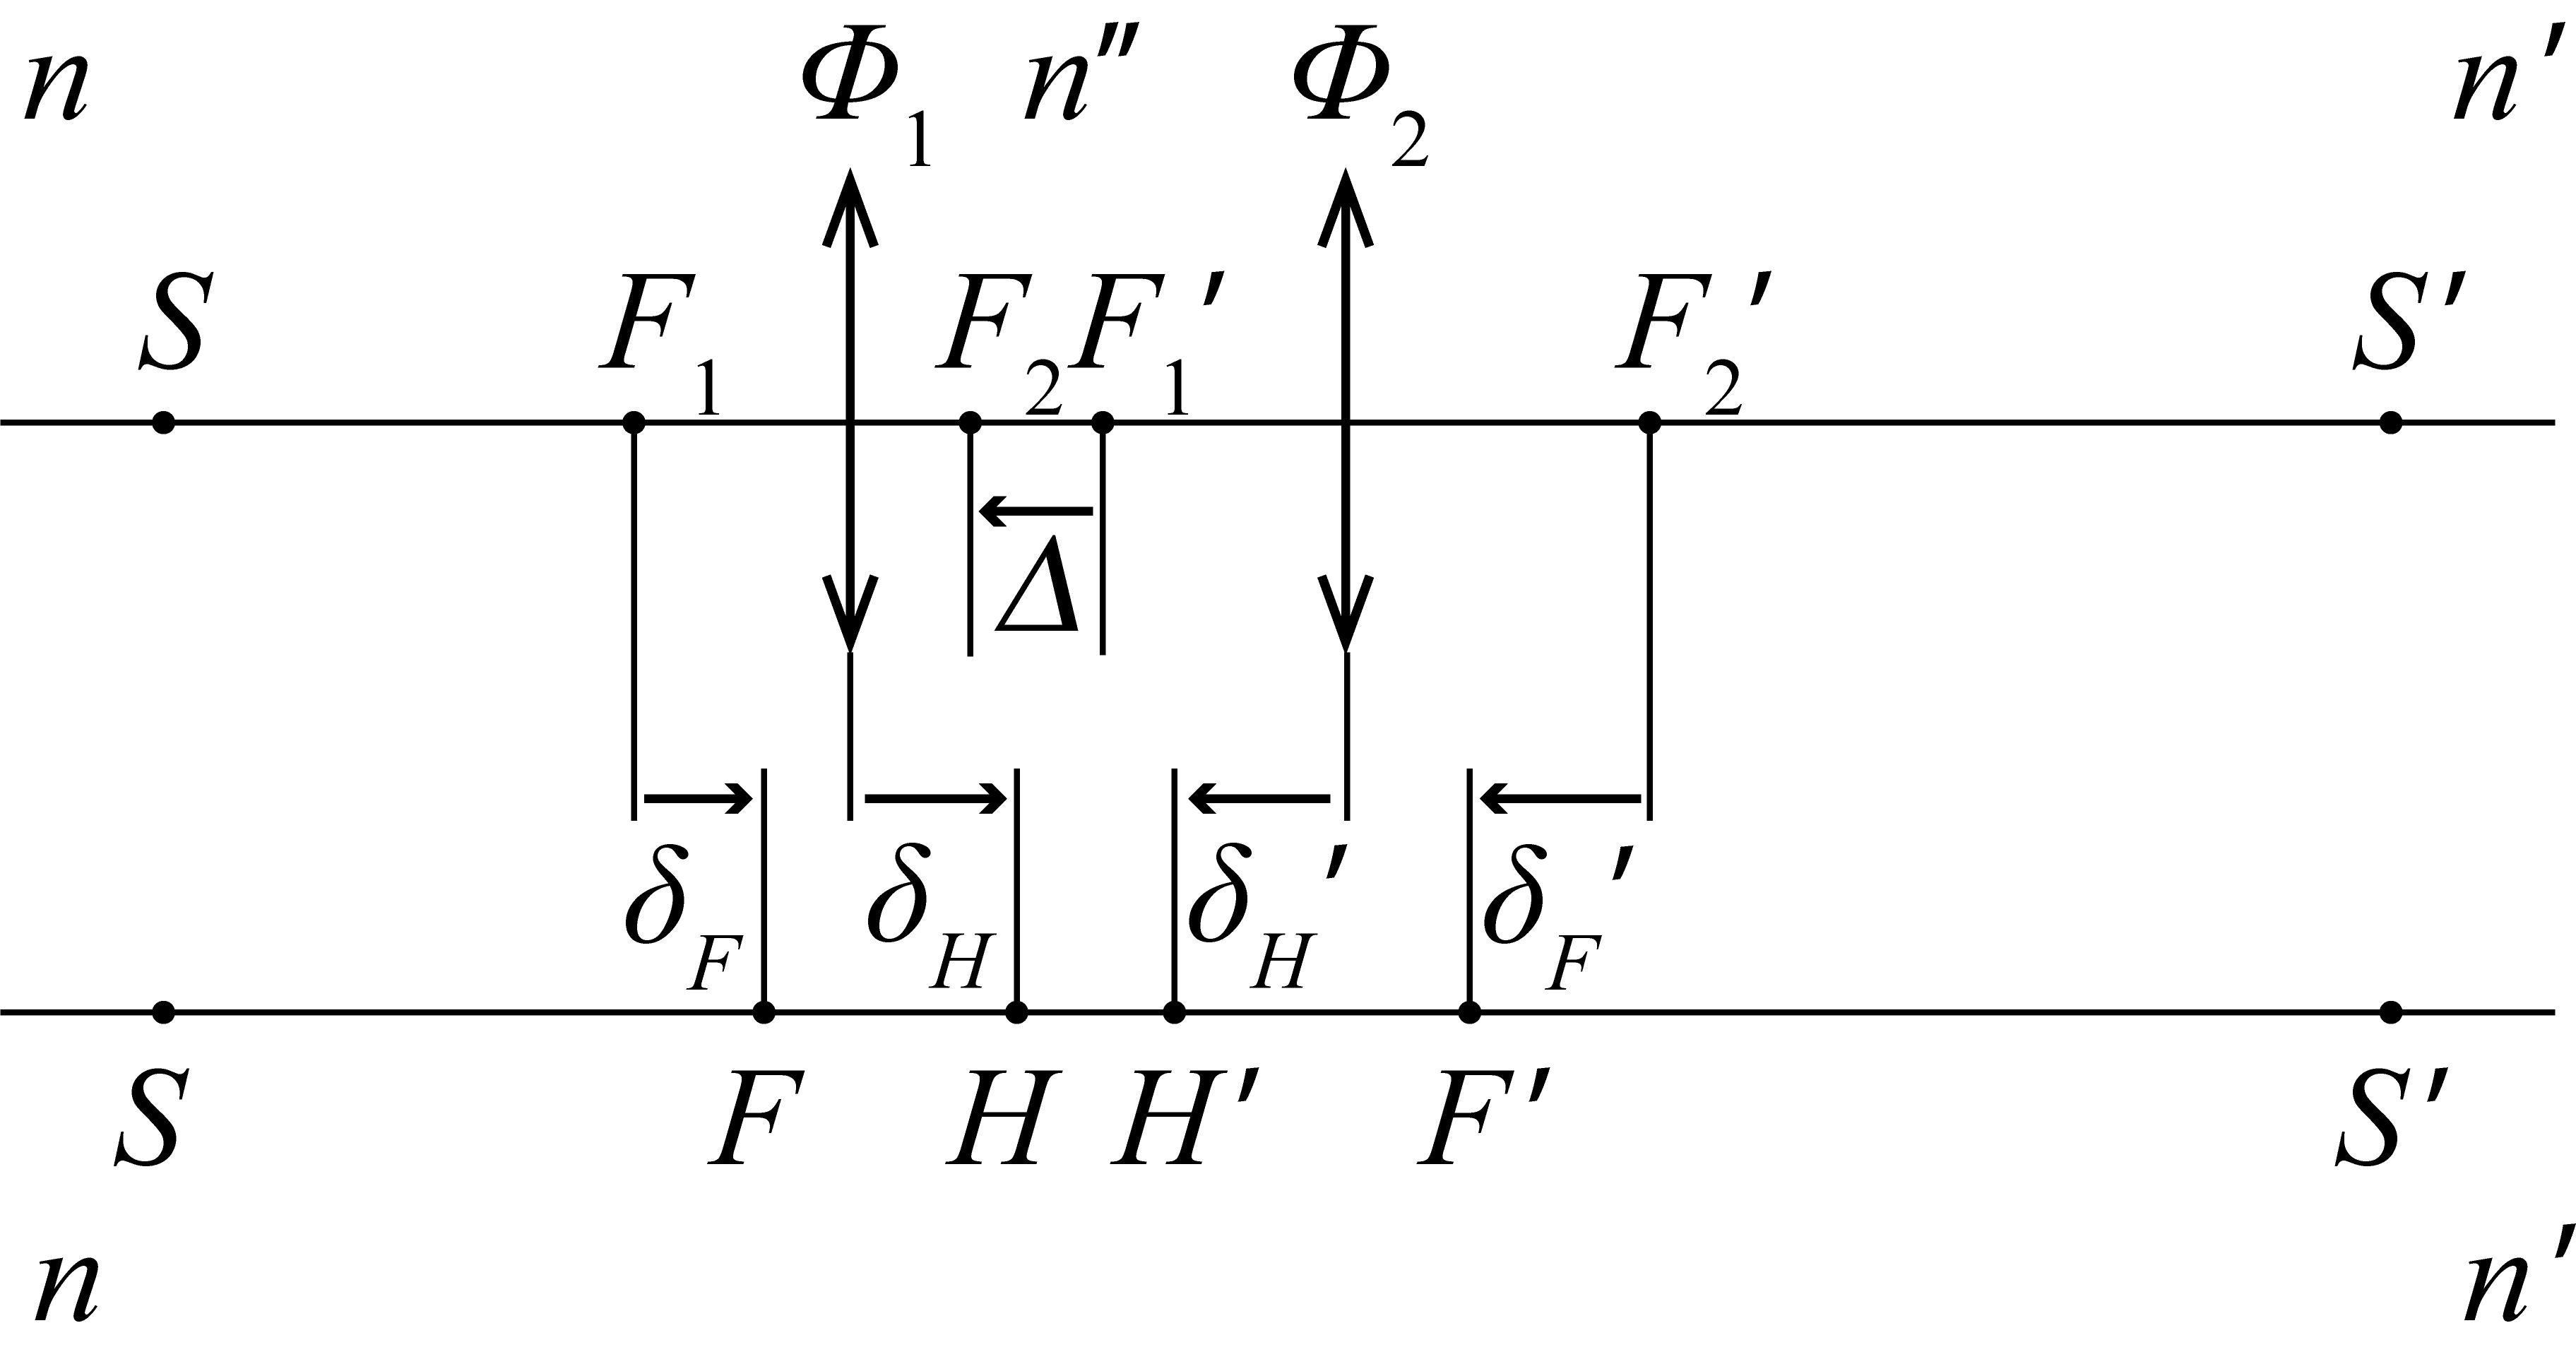
\includegraphics[width=8cm]{image/5-7-6.png}
\caption{透镜组}
\end{wrapfigure}
如图,\,如果考虑\emph{厚透镜}(thick lens)模型,\,或者更普遍地讨论两个薄透镜相隔一定距离放置的情况.\,那么一般把前透镜像方焦点到后透镜物方焦点的以传播方向为正的距离即为\emph{光学距离}(optical distance).\,即\(\varDelta=\overline{F_1' F_2}\),\,两透镜间距离:
\[d=f_1'+f_2+\Delta\]

上图的\(\varDelta\)实际上取负,\,事实上当\(\varDelta=-f_1'-f_2\)时变为密接的情形,\,而\(\varDelta\)增大也代表着\(d\)增大.\,我们写出此时的成像物像距公式:
\[\frac{n}{s}+\frac{n''}{s_1'}=\varPhi_1\]
\[\frac{n''}{s_2}+\frac{n'}{s'}=\varPhi_2\]
\[s_1'+s_2=d=\frac{n''}{\varPhi_1}+\frac{n''}{\varPhi_2}+\varDelta\]
得到:
\[(s-f_1-\frac{f_1f_1'}{\varDelta})(s'-f_2'-\frac{f_2f_2'}{\varDelta})=\frac{f_1f_1'f_2f_2'}{\varDelta^2}\]

上式即成像公式的牛顿形式.\,而由牛顿型的放大率公式:
\[\beta=(-\frac{f_1}{s-f_1})(-\frac{s'-f_2'}{f_2'})\]

代入上式可得:
\[\beta=-\frac{-\frac{f_1f_2}{\varDelta}}{s-f_1-\frac{f_1f_1'}{\varDelta}}=-\frac{s'-f_2'-\frac{f_2f_2'}{\varDelta}}{-\frac{f_1'f_2'}{\varDelta}}\]

从中可以发现,\,这个成像公式恰恰等价于一个物像距的零点不位于两个透镜光心.\,而两侧的焦点也不与原来的焦点重合的成像系统,\,仍然有其焦距为:
\[f=\overline{FH}=-\frac{f_1f_2}{\varDelta}\;,\; f'=\overline{H'F'}=-\frac{f_1'f_2'}{\varDelta}\quad ;\quad f:f'=n:n'\]

而各个特征点位移为:
\[\delta_F=\overline{F_1F}=-\frac{f_1f_1'}{\varDelta}\quad;\quad \delta_F'=\overline{F'F_2'}==-\frac{f_2f_2'}{\varDelta}\]
\[\delta_H=\overline{O_1H}=-\frac{f_1d }{\varDelta}\quad;\quad \delta_H'=\overline{H'O_2}=-\frac{f_2' d}{\varDelta}\]

其中\(H\)被称作等效光学系统的物方主点,\,\(H'\)被称作等效光学系统的像方主点.以上公式的理解中如果\(\varDelta<0\),\,那么各个量就都是正的.\,图画的正是这个情况.\,此时的成像规律,\,可以认为是在\(H\)处具有光焦度为\(\varPhi=-\dfrac{n''\varDelta}{f_1'f_2}\)的透镜,\,再把其直接成像的结果进行一个平移,\,平移距离即为两个主点间距\(\overline{HH'}\).\,正是因为这个原因,\,考虑多次成像系统的复合时可以再把两个光具等效的光学系统再与第三个光具按照以上公式再进行等效,\,直到化为最基础的成像公式的情形.

\section{理想成像系统}
把傍轴成像系统的特性进行数学上的抽象与大胆的推广,\,我们得到了理想光具组成像系统.\,它是一个全空间中点到全空间中点的可逆映射:
\[\mathcal{I}:\; S\to S'\quad,\quad S\in\mathbb{R}^3\cup\{\infty\}\]

在这个映射中无穷远点也是有意义的.\,一般正负无穷远处的点其实没有区别(发出平行光),\,不同的无穷远点根据其发出的光与主光轴的夹角定义.\,而理想光具组需要有以下特征:
\begin{enumerate}
	\item 主光轴必须被映射到主光轴.
	\item 映射关于主光轴对称.\,可以认为是一个平面上的映射绕主光轴旋转而生成的.\,
	\item 保直线,\,平面的形状.\,直线点集与平面点集映射到直线与平面.
\end{enumerate}

仅这三个条件,\,足以把映射的性质确定到仅含极少参数,\,也就是我们上一节介绍的成像系统.\,这是因为可以根据以上定义证明以下性质(作为思考题请读者自己思考):
\begin{enumerate}
	\item 垂直于主光轴的平面一定被映射到垂直于主光轴的平面.
	\item 在垂直于光轴的平面之间的映射是简单的放缩变换(横向放大率为常数).
	\item 不同的物距的横向放大率,\,要么始终保持为常数,\,要么连续,\,单次地取遍任意正负值.\,前者称为\emph{望远系统}(afocal system).
\end{enumerate}

所以我们把这个映射的性质总结为在一个过主光轴的平面内的问题,\,这个平面称为\emph{子午面}(meridinal plane),\,只需要物像距公式和放大率公式两个成像公式.\,而定义若干的辅助点,\,辅助面可以帮我们有效的研究非望远系统的性质.\,这些点与面被称作\emph{基点}(cardinal point)与\emph{基面}(cardinal plane).\,除了望远系统,\,所有理想光具组成像都有两对关键基点,\,它们都是主光轴上的特殊点,\,而有基面即过基点的垂直于主光轴的平面,\,代表特殊的物像距处物像高的所有可能性.\,它们是:
\begin{description}
	\item[{\hei 主点(principal points)}:] 横向放大率为\(1\)的那对共轭点即为物方主点与像方主点.
	\item[{\hei 焦点(focal points)}:] 横向放大率发散(\(\infty\))时,\,物方为物方焦点,\,像方为无穷远点.\,横向放大率为\(0\)时,\,物方为无穷远,\,像方则为像方焦点.
\end{description}

有了以上定义以后,\,便可以用作图法确定成像公式.

\subsection{作图法}
作图法的基础是以下两个简单结论:
\begin{itemize}
	\item 凡入射到物方主平面上一点的光线必然在像方主平面上等高处出射.
	\item 平行光入射,\,出射光聚焦于像方焦平面上某点.\,物方焦平面上一点入射,\,则出射平行光.\,更特别地,\,经过物方焦点的光线出射光平行于主光轴,\,平行于主光轴的光入射后出射光经过像方焦点.
\end{itemize}
\begin{figure}[H]
\centering
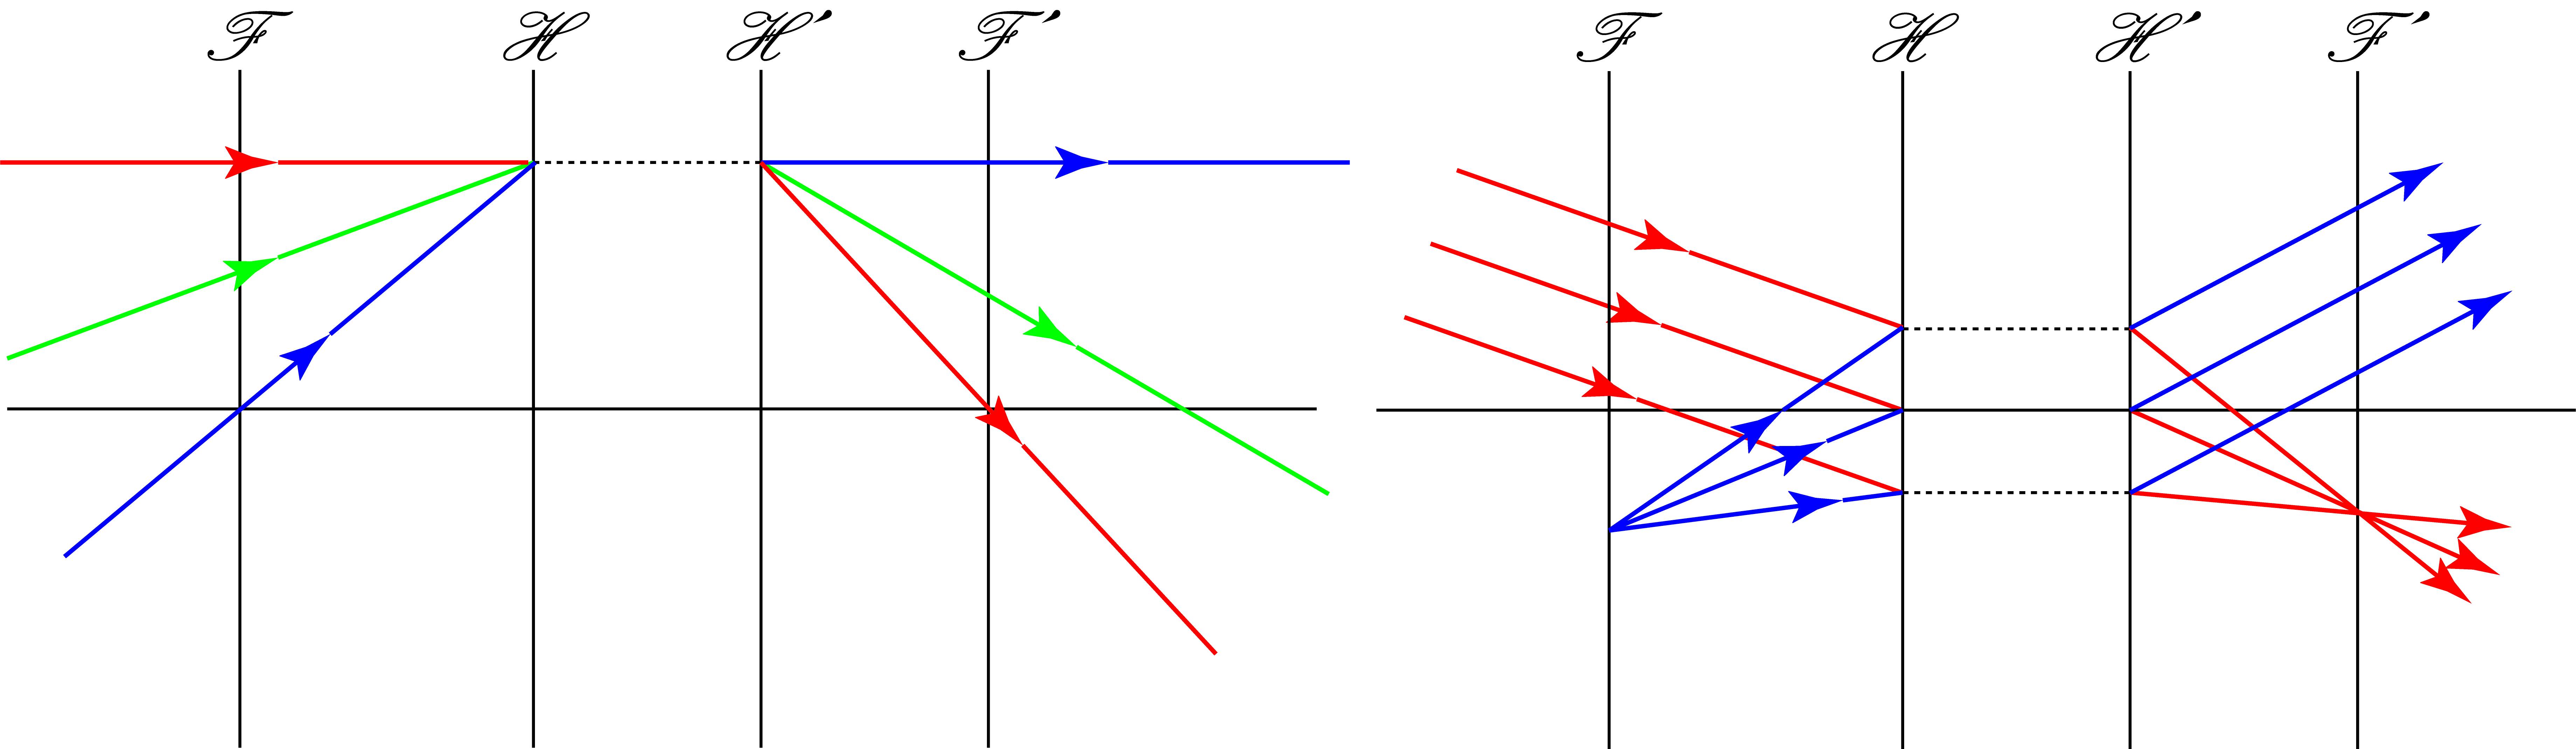
\includegraphics[width=0.9\textwidth]{image/5-7-7.png}
\caption{特殊光线}
\end{figure}

通过以上特殊光线我们可以确定任意一条入射光线对应的的出射光线,\,也能进一步明确到每一个物对应的像的位置.\,如下图左所示.\,给出一条入射光线\(AB\).\,如果它入射到物方主面上的\(B\)点.\,那么必然从像方主面上的等高\(C\)点出射.\,于是做出两条辅助光线:\,一是从入射光线经过的物方焦面上的点作平行与主光轴的光线(红色),\,那么我们很容易找到它的出射光线.\,那么原光线与此特殊光线必然出射平行光而找到出射\(CD\)的方向.\,二是也可以做出过物方焦点且与\(AB\)平行的辅助入射光线.\,也可以找到它的出射光线从而确定出\(CD\)来.\,而如果要找物\(S\)的像\(S'\)的位置,\,也是利用特殊的光线确定的,\,如下图右.\,通过几何上三角形\(1\)与\(2\),\,\(3\)与\(4\)的相似关系:
\[\frac{y}{-y'}=\frac{x}{f}\quad ;\quad \frac{-y'}{y}=\frac{x'}{f'}\]

整理即为牛顿型的成像公式:
\[xx'=ff'\quad ;\quad \beta=-\frac{f}{x}=-\frac{x'}{f'}\]

再利用\(s=f+x\),\,\(s'=f'+x'\)可以确定从主面出发计算物像距的对应高斯型成像公式:
\[\frac{f}{s}+\frac{f'}{s'}=1\quad ;\quad \beta=-\frac{fs'}{f's}\]
\begin{itemize}
	\item 凡入射到物方主平面上一点的光线必然在像方主平面上等高处出射.
	\item 平行光入射,\,出射光聚焦于像方焦平面上某点.\,物方焦平面上一点入射,\,则出射平行光.\,更特别地,\,经过物方焦点的光线出射光平行于主光轴,\,平行于主光轴的光入射后出射光经过像方焦点.
\end{itemize}
\begin{figure}[H]
\centering
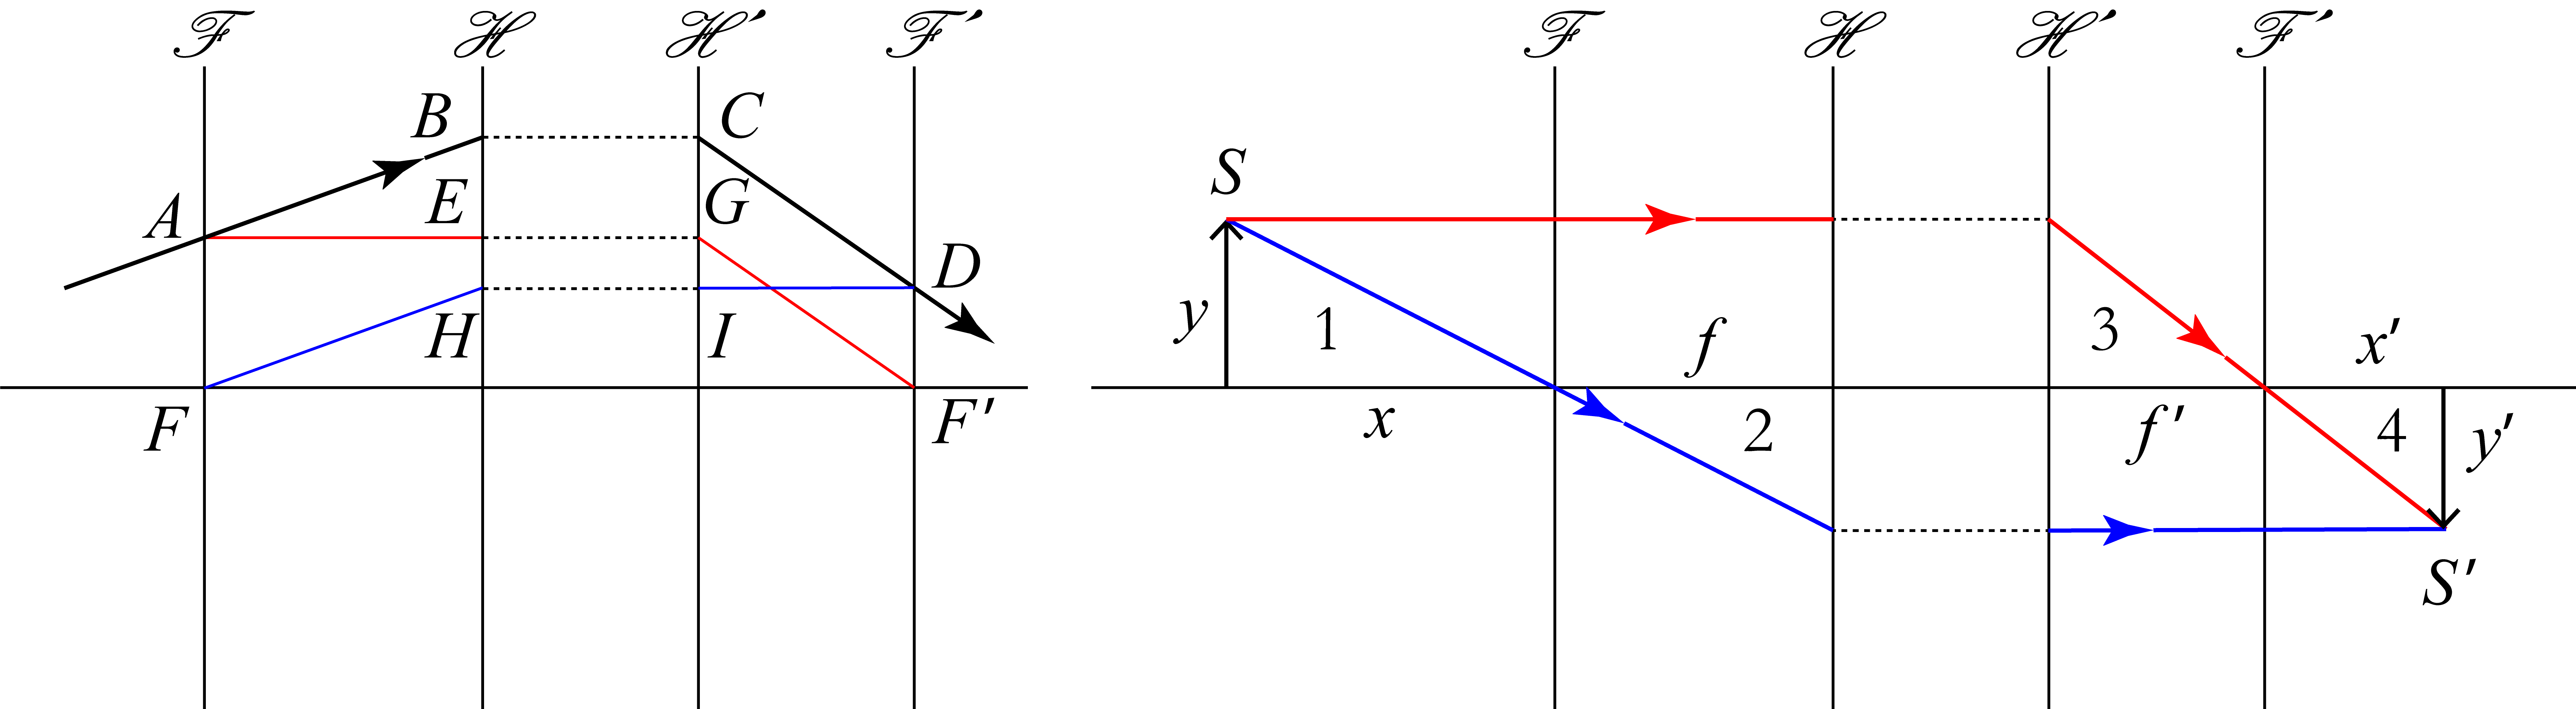
\includegraphics[width=0.9\textwidth]{image/5-7-8.png}
\caption{共轭线与共轭点}
\end{figure}

\subsection{基点基面性质}
\begin{wrapfigure}[11]{o}[-10pt]{8cm}
\centering
\vspace{0cm}
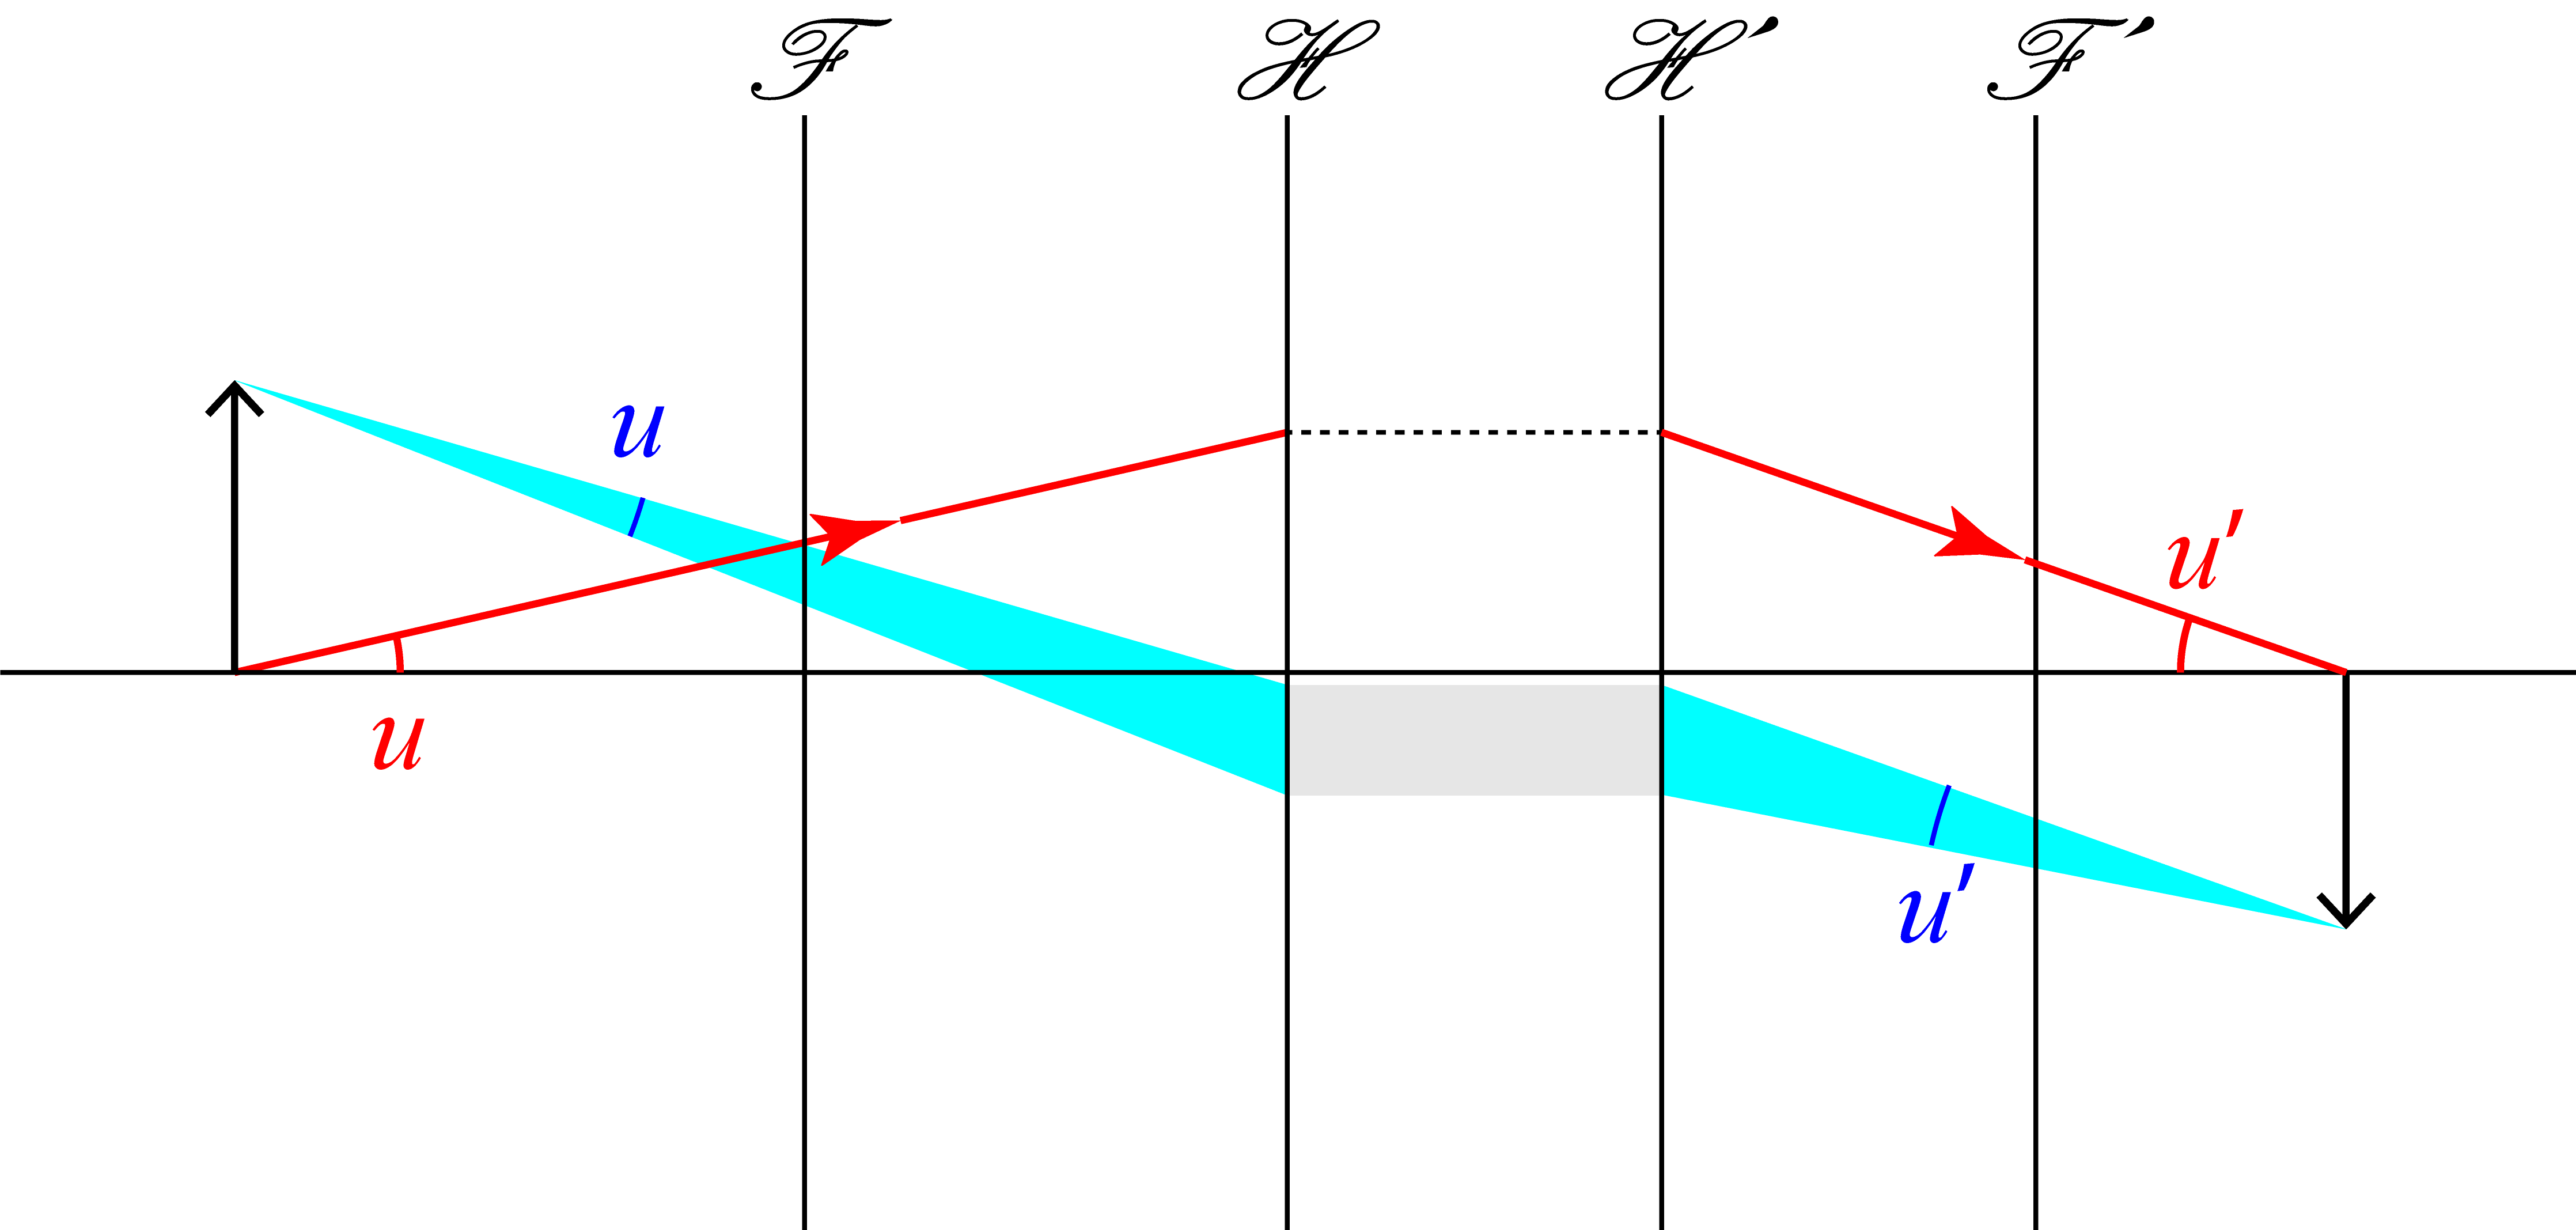
\includegraphics[width=8cm]{image/5-7-9.png}
\caption{角度的放大}
\end{wrapfigure}
在实际傍轴成像过程中还有一个我们比较关系的量.\,就是在一定物距与对应的像距处的成像的\emph{角度放大率}(angular magnification).\,它被定义为物点傍轴发出一个顶角为\(u\)小角的光锥时\footnote{这里考虑平面问题,\,空间情形可以比较类似地讨论,\,此时应该考虑立体角.},\,成像处对应的光锥顶角\(u'\)的放大率.\,在傍轴的小角近似下,\,也可以定义为过零物像高处的共轭点的共轭光线的夹角比.\,后一个定义能产生正负号,\,我们采用后一种定义(右图中红色的角).
\[B=\frac{u'}{u}\]

而如果考虑的是理想光具组情形,\,我们可以将上式写为更严格的形式:
\[B=\frac{\tan u'}{\tan u}\]

从图中可以发现,\,这样定义角度放大率后它与物像距的关系从图中可以写出:
\[s\tan u=s'\tan (-u')\quad\Rightarrow\quad B=-\frac{s'}{s}=\frac{f'}{f}\beta\]

考虑牛顿公式\(xx'=ff'\),\,除去焦点与焦面,\,还有有四种独特的物像距分别具有独特的性质.\,它们对应的主光轴上的点与平面都被称作基点与基面.\,而各个点性质如下:

\begin{description}
	\item[\hei 主点(principal points)]:\,\(x=-f,\,x'=-f'\Rightarrow\beta=1\).\,成等大正立像.
	\item[\hei 二倍焦距点]:\,\(x=f,\,x'=f'\Rightarrow\beta=-1\).\,成等大倒立像.
	\item[\hei 节点(nodal points)]:\,\(x=-f',\,x'=-f\Rightarrow B=1\).\,角放大率为一.
	\item[\hei 物像距等值点]:\,\(x=f',\,x'=f\Rightarrow B=-1\).\,角放大率为负一.
\end{description}

其中节点概念在光学测量中有重要的作用.\,它的特点是,\,入射到物方节点\(N\)光线,\,方向不改变地从像方节点\(N'\)出射.\,注意到这个角放大率为一的事实也仅仅在物像距为节点时能够取到.\,节点也是经常讨论的关键基点

\begin{wrapfigure}[9]{o}[-10pt]{7cm}
\centering
\vspace{0cm}
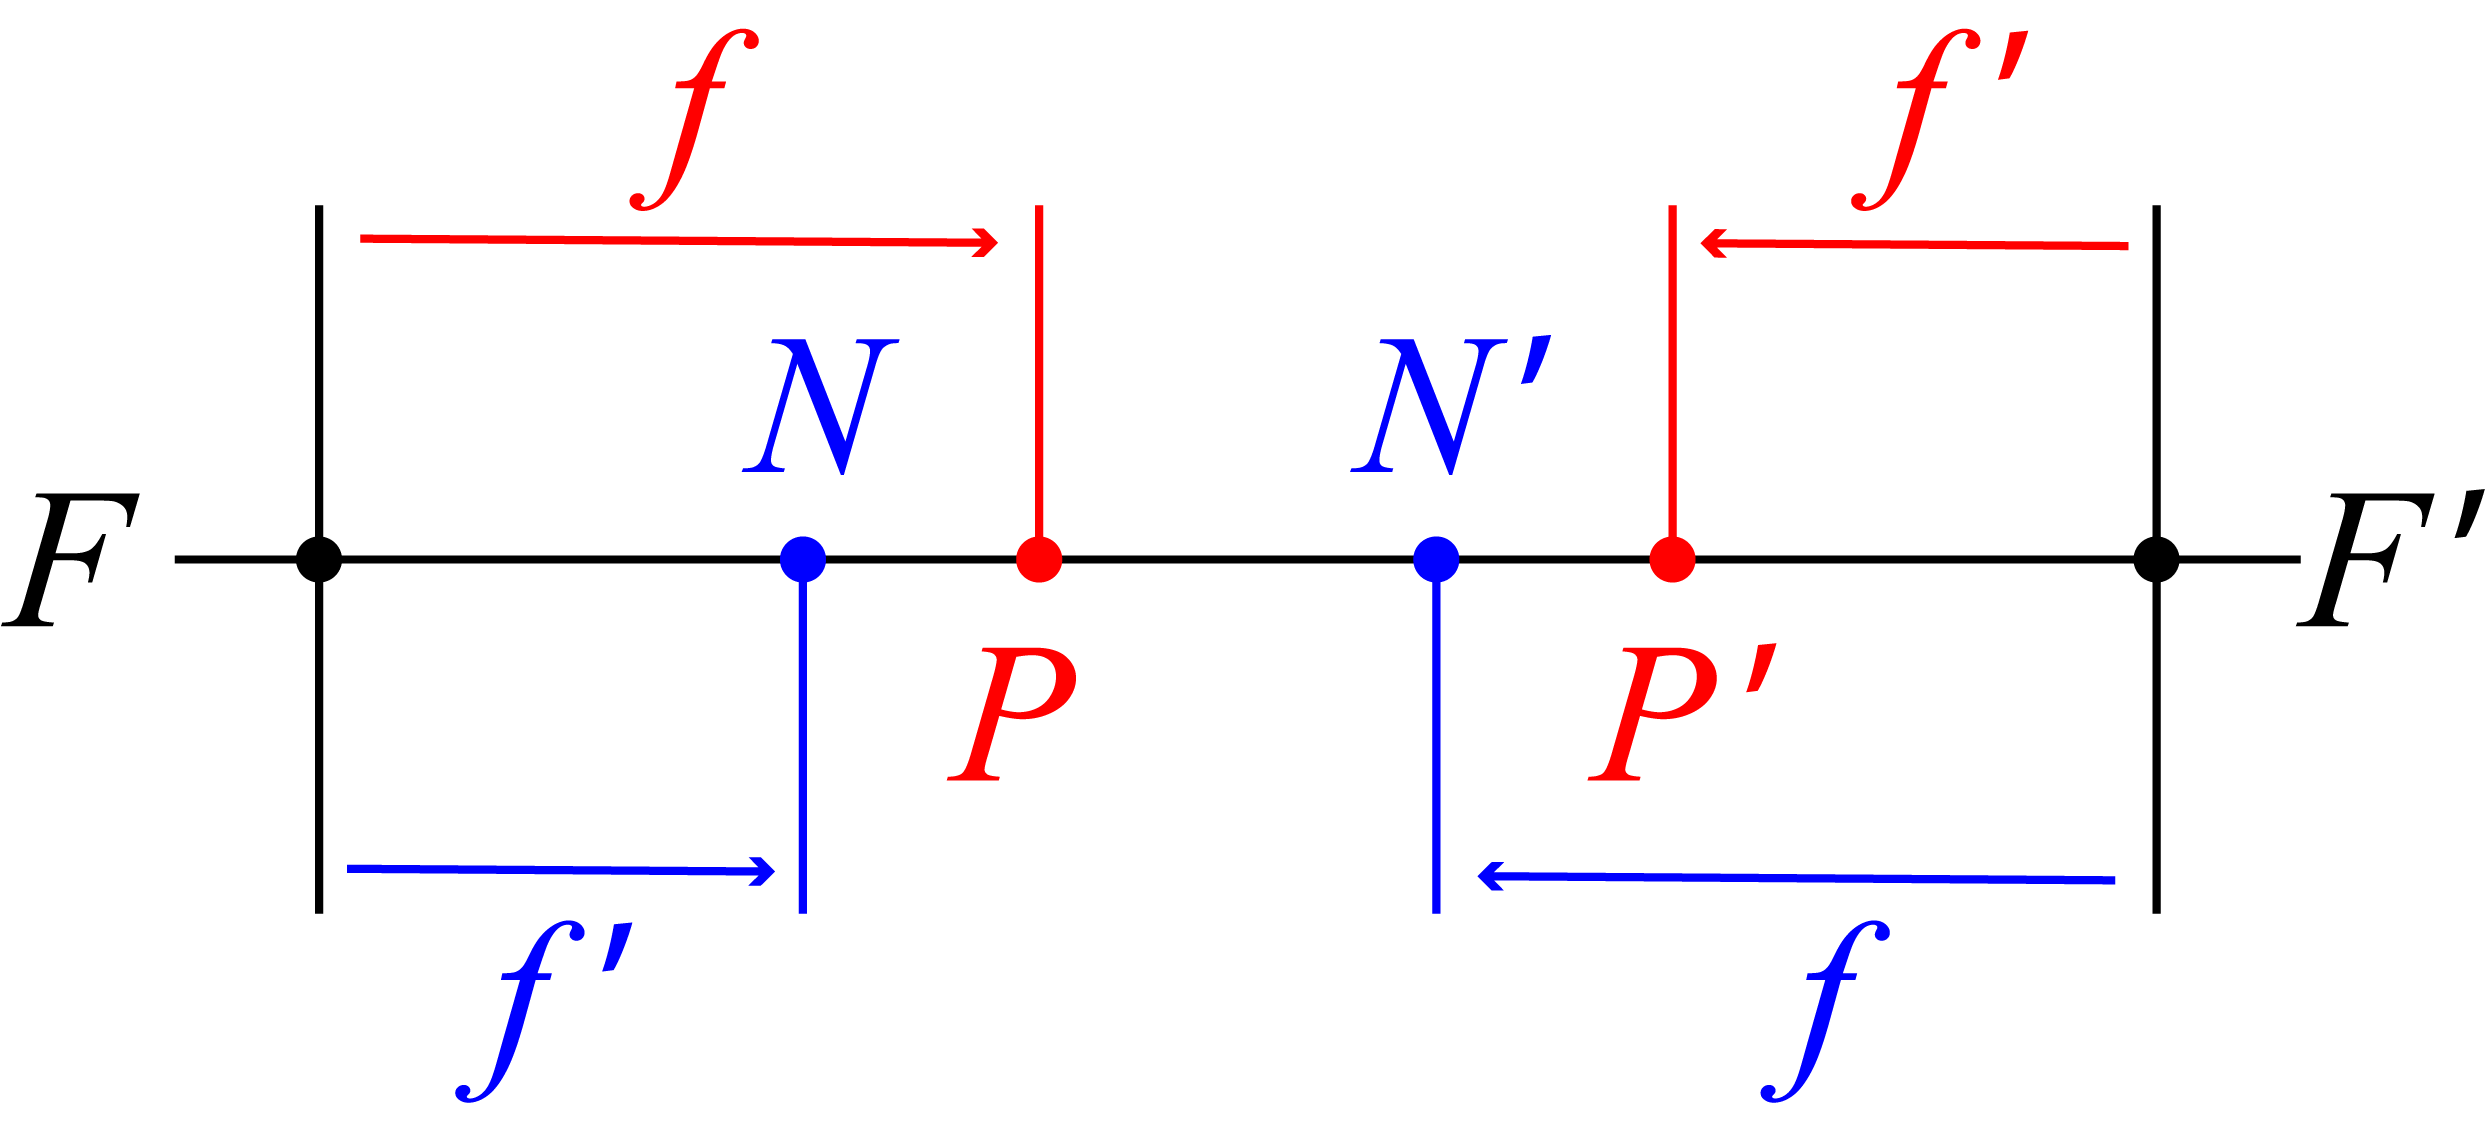
\includegraphics[width=7cm]{image/5-7-10.png}
\caption{三对关键基点}
\end{wrapfigure}
我们可以这么理解这三对基点的关系,\,\(xx'=ff'\)提示我们,\,只需要知道\(ff'\)乘积整体的值便可以确定物像距之间的对应关系,\,而两者之比\(f:f'=n:n'\)\footnote{这个表达式的普遍性参考下一节与下一章.}则告诉我们放大率的信息.\,实际上就是分别确定物方主点在焦点后方多远,\,像方主点在像方焦点前多远.\,而把这两个距离对换,\,就变成了对应的节点位置.\,换句话说,\,如果把两焦点的中点看做对称中心,\,则两个主点对这个点中心反演就到了两个节点.

这也就是说,\,如果物方像方折射率相等(这实际上是较常遇到的情况),\,那么也就没有\(f\)与\(f'\)的区别,\,那么上面列举的四对基点退化为两对.\,节点与主点必然重合,\,横向放大率与角度放大率都是\(1\).\,而二倍焦距处的那两个共轭点(物方\(2F\)点,\,像方\(2F'\)点,\,成像系统常称\(4F\)系统),\,物像互为倒立关系,\,横向放大率与角度放大率为\(-1\).

\subsection{实例与望远系统}
球面折射,\,即可以傍轴近似为两个主点重合到光心(与两节点都不重合),\,物像方焦距分别为:
\[f=\frac{nR}{n'-n}\quad;\quad f'=\frac{n'R}{n'-n}\]

如果\(R\to \infty\),\,\(\varPhi\to 0\).\,即平面折射,\,那么成像系统化为望远系统.\,此时物像距为简单线性关系,\,横向放大率处处一样:
\[\frac{s'}{s}=-\frac{n'}{n},\,\beta=1\]

横向放大率为\(1\)是系统沿平面界面平移对称的结果.

\begin{wrapfigure}[11]{o}[-10pt]{8cm}
\centering
\vspace{0cm}
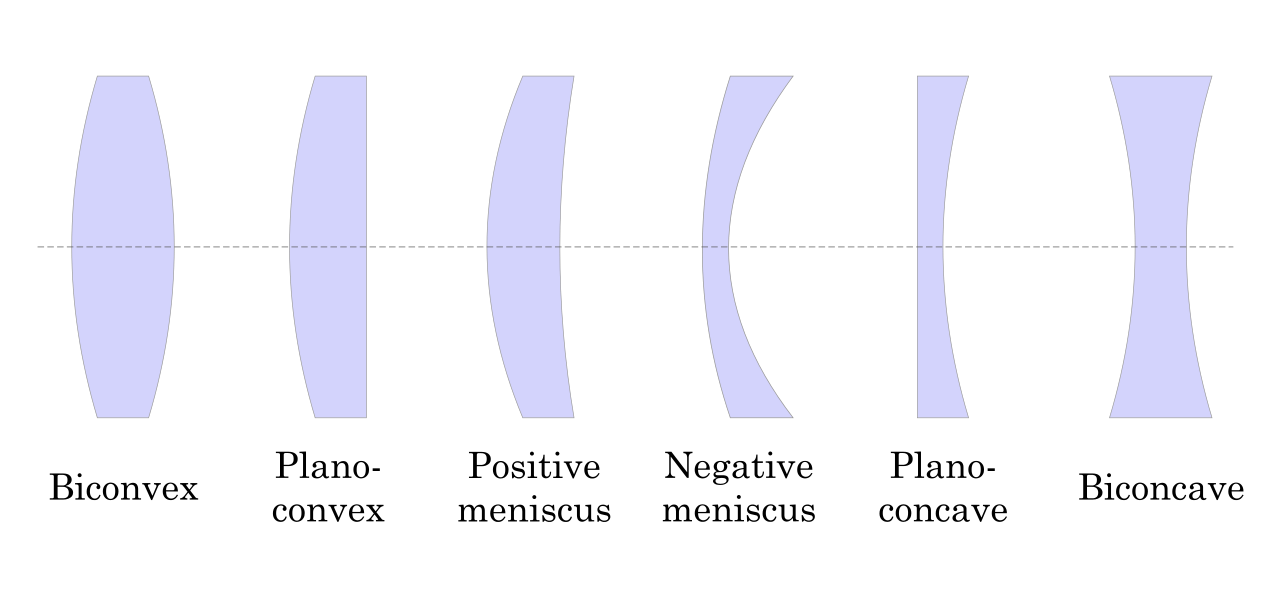
\includegraphics[width=8cm]{image/5-7-11.png}
\caption{透镜种类}
\end{wrapfigure}
而对于更复杂而常见的厚透镜系统,\,一般我们做如图所示的分类.\,即分为\emph{双凸透镜}(biconvex lens),\,\emph{双凹透镜}(biconcave lens),\,\emph{平凸透镜}(planoconvex lens),\,\emph{平凹透镜}(planoconcave lens),\,\emph{正弯月透镜}(positive meniscus lens)与\emph{负弯月透镜}(negative meniscus lens).\,一般置于折射率为\(1\)的空气中,\,透镜折射率计为\(n\),\,厚度记为\(d\).\,则有以下\emph{磨镜者公式}(lensmaker's equation):
\[\varPhi=\frac{1}{f}=(n-1)[\frac{1}{R_1}+\frac{1}{R_2}-\frac{(n-1)d}{nR_1R_2}]\]

推导参考之前的证明过程.\,注意此处的焦距是要从两个主面开始计算的,\,而两个主面的位置一般并不会与左右两折射面与主光轴交点重合.\,而是相距:
\[\overline{HH'}=\frac{d(\varDelta+f_1+f_2')}{\varDelta}\quad;\quad \varDelta=d-f_1'-f_2\]
\[f_1=\frac{R_1}{n-1}\quad ;\quad f_1'=\frac{nR_1}{n-1}\]
\[f_2=\frac{nR_2}{n-1}\quad ;\quad f_2'=\frac{R_2}{n-1}\]

我们讨论四种特殊的情形.\,一是\(R_1+R_2=d\)的情形.\,此时恰有:
\[\varDelta+f_1+f_2'=d-(f_1'-f_1)-(f_2-f_2')=d-R_1-R_2=0\]

即两个主点重合.\,其实,\,两个主点必然重合到左右球面的公共球心.\,这是因为如果入射光线过这个点,\,那么出射光线方向恰好不改变,\,必然也过这个点,\,从而这个点是节点,\,而对称成像系统(物像方折射率相等,\,焦距相等)的主点与节点时重合的.\,从而主点也在这里.\,只需要确定焦距便可以决定的所有特征.\,它由下式给出:
\[f=\frac{nR_1R_2}{(n-1)d}\]

第二种情况是\(\varDelta=0\),\,即\(\dfrac{nR_1}{n-1}+\dfrac{nR_2}{n-1}=d\).\,此时光焦度变为零,\,成像系统成为望远系统.\,望远系统由于各种量的发散性,\,其物像距关系与放大率都必须重新讨论.\,如图\ref{fig5-7-12},\,我们把物距\(x\)仍然计做物到左折射球面左焦点的距离,\,而像距\(x'\)仍计做像到右折射球面右焦点的距离,\,有:
\[xx_1'=f_1f_1'\quad ;\quad \beta_1=-\frac{f_1}{x}\]
\[x_2x'=f_2f_2'\quad ;\quad \beta_2=-\frac{x'}{f_2'}\]

再考虑到两次成像有\(x_1'=-x_2\),\,得到:
\[\frac{x'}{x}=-\frac{f_2f_2'}{f_1f_1'}=-\frac{R_2^2}{R_1^2}\]
\[\beta=-\frac{f_2}{f_1'}=-\frac{R_2}{R_1}\]

可见物像距间有线性关系,\,而横向放大率是一个常数.\,我们也定义\emph{纵向放大率}(longtitudinal magnification):
\[\varXi=\frac{\ud x'}{\ud x}=-\beta^2\]

纵向放大率的大小为横向放大率的平方,\,这个结论其实对对称薄透镜也是适用的(请读者证明),\,此时物像距关系非线性,\,故应采用严格的导数来定义局域放大率.

\begin{figure}[H]
\centering
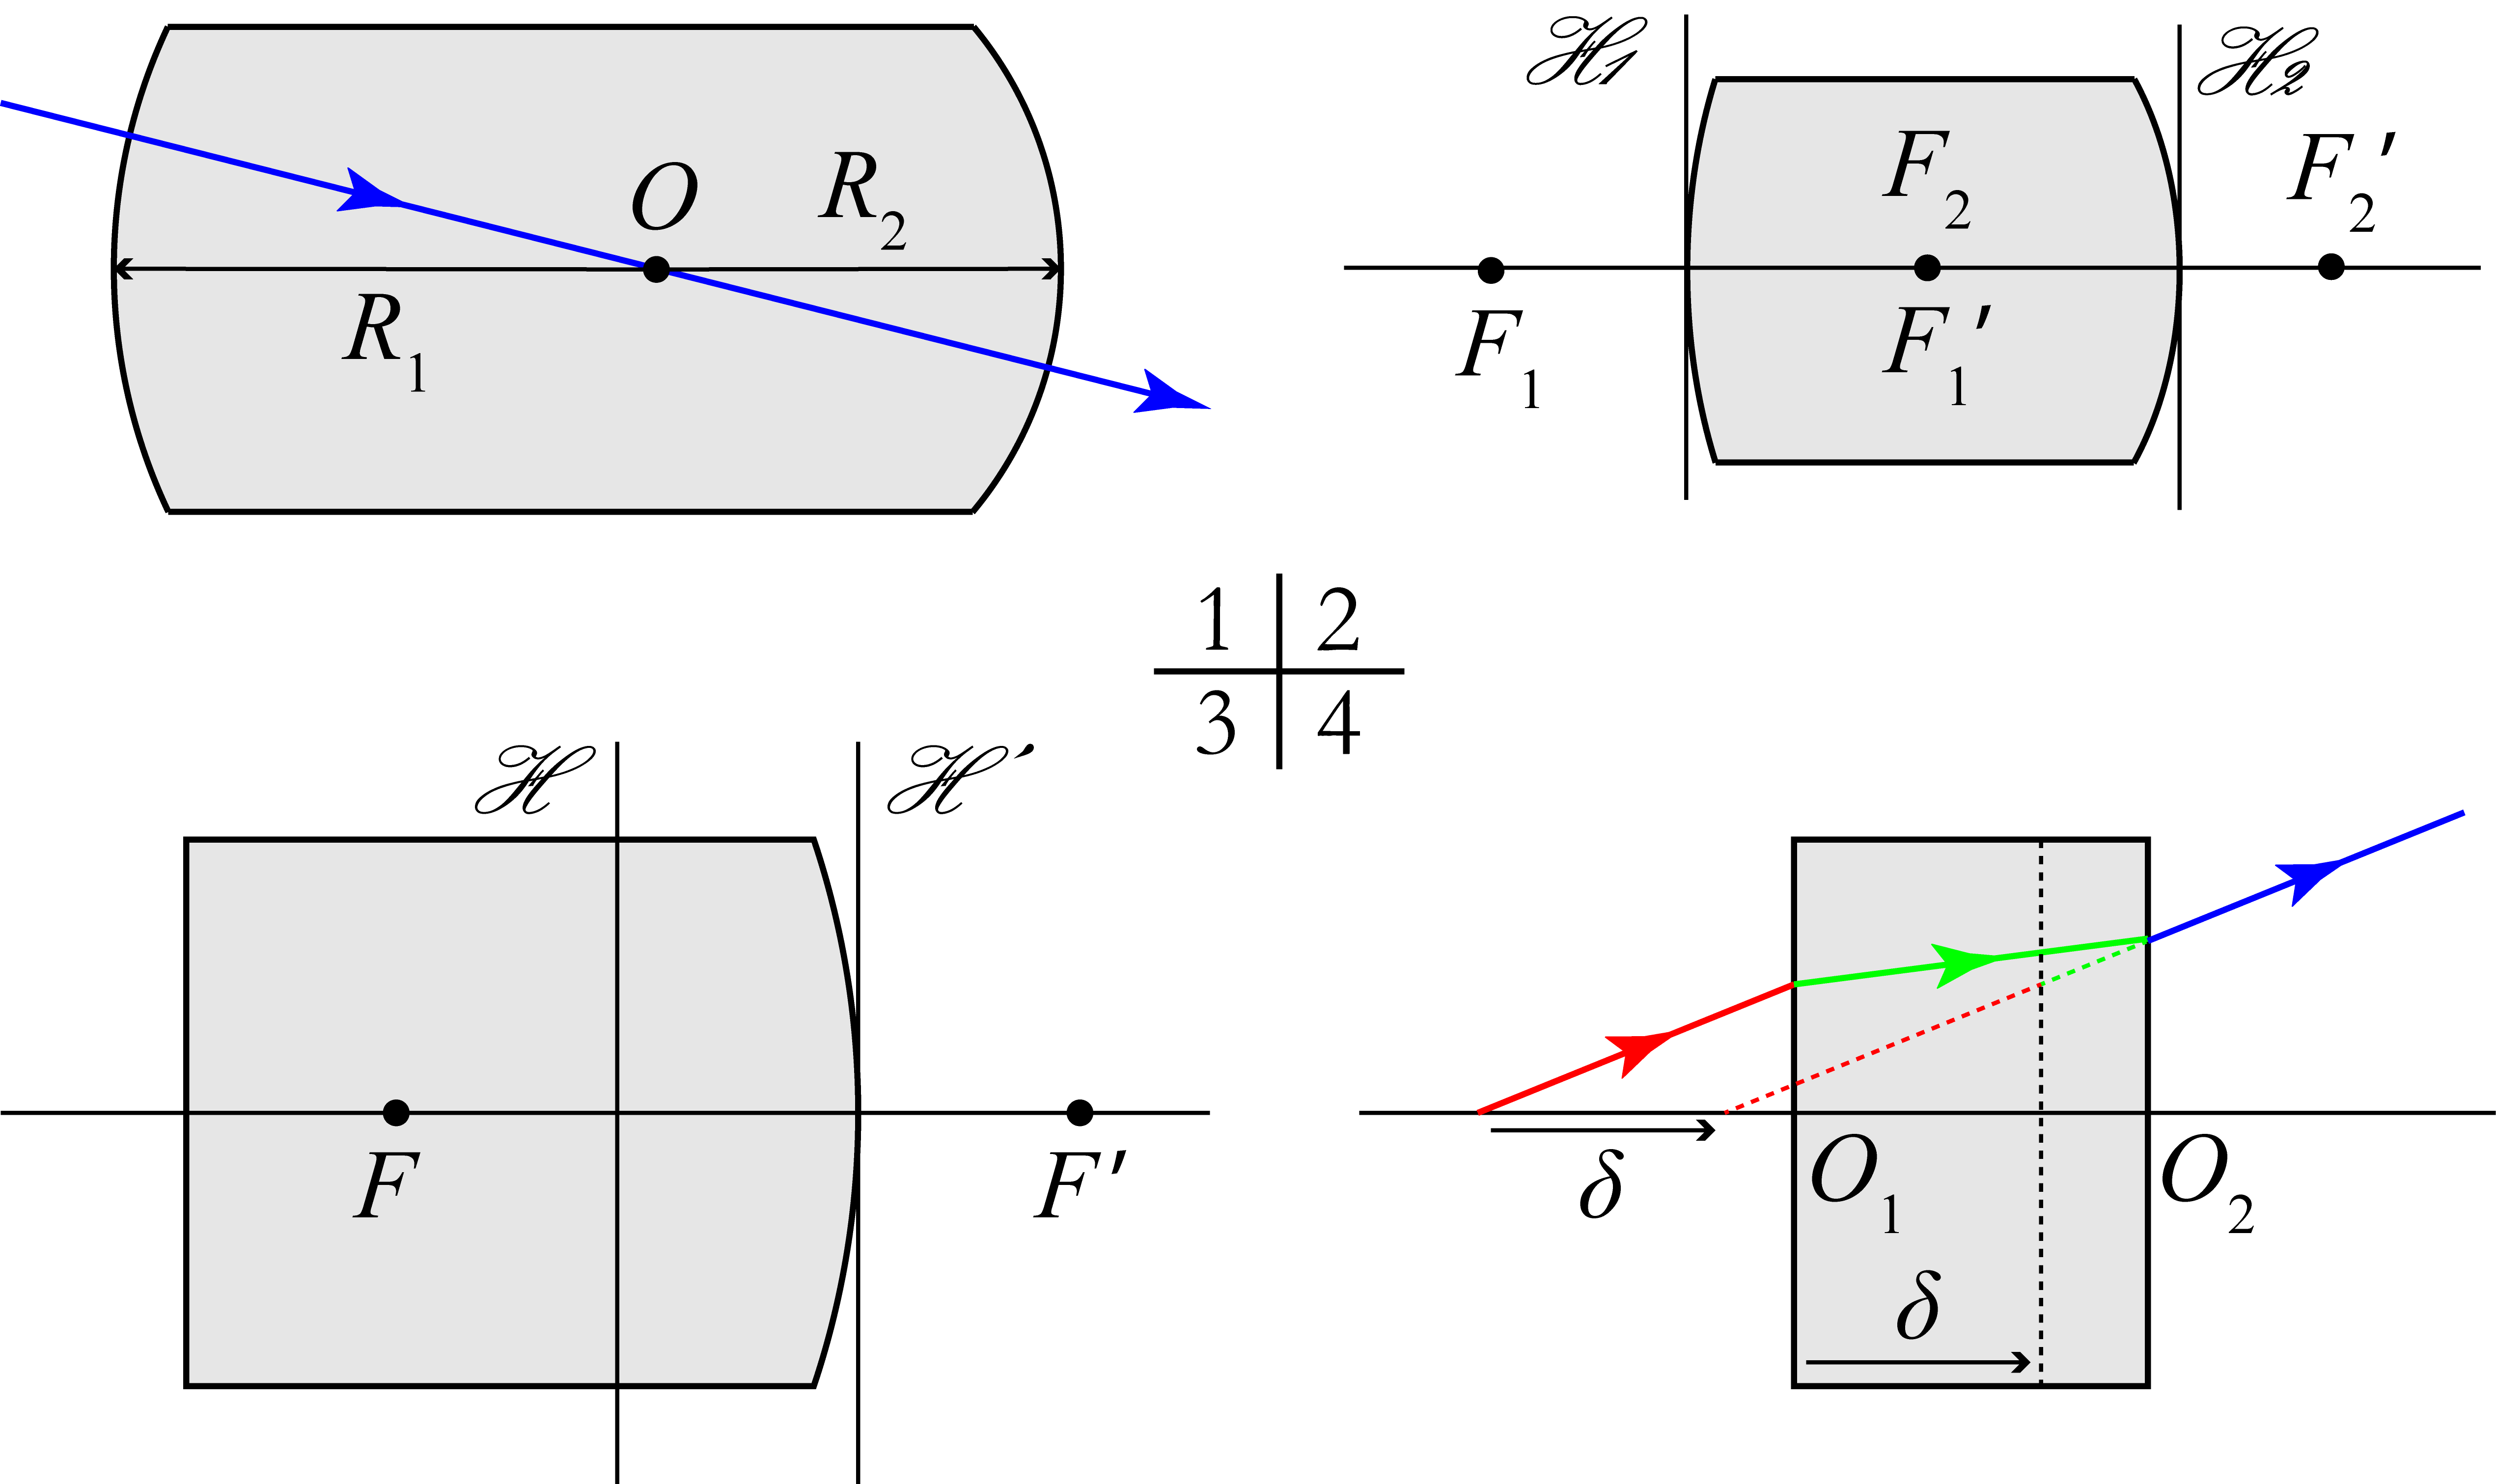
\includegraphics[width=0.7\textwidth]{image/5-7-12.png}
\caption{四种特殊厚透镜}
\label{fig5-7-12}
\end{figure}

第三种情况是有一个球面退化为平面的情况,\,此时各公式也因为发散而实效.\,如\(R_1\to\infty\)成为平面.\,如图\ref{fig5-7-12},\,我们可以根据此时成像系统的特征确定等效的各基点.\,像方焦点显然位置仍然在右折射面像方焦点的位置,\,这是因为平行光经过平面折射仍然是平行光,\,就应该会聚在这个焦面上.\,而像方主面也仍然在右折射面顶点处.\,这可以从平行于主轴的光线的传播确定出来.\,从而焦距即为右球面的像方焦距\(f=\dfrac{R_2}{n-1}\).\,物方主面位于像方主面经左平面折射成像的位置,\,而物方焦点还在其左侧距离\(f\)处,\,这些都很容易理解,\,留给读者思考其原因.

最后一种情况是两个球面都退化为平面的情况.\,这是不仅公式发散需要重新计算,\,它的结果还是一个望远系统.\,事实上我们可以考虑傍轴的几何光学,\,用简单的\emph{光线追迹法}(ray-tracing method),\,我们发现如果把玻璃砖的厚度进行压缩到\(d/n\),\,那么所有光线都变成了直线传播.\,从而物就重合到了像.\,所以我们发现此时的物像映射实际上就是一个固定距离\(\delta=\dfrac{n-1}{n}d\)的平移,\,其横向纵向放大率都是\(1\).

\section{更多讨论*}
\subsection{理想成像本质}
理想光具组是一种十分强大的工具,\,但一些普遍的规律仍然悬而未决:\,为什么根据光线的对应性能把成像确定到如此小的范围.\,物像方的焦距为什么总是与折射率正相关,\,同正同负.\,而各个放大率间的关系又是如何.\,所以我们提出理想成像的数学本质抽象:\,射影变换.

首先是数学上有著名的\emph{射影几何基本定理}(fundamental theorem of projective geometry):

\begin{quote}
\hei 实线性空间上的\emph{共线性变换}(collineation)是更高维度内的\emph{射影变换}(projection).
\end{quote}

\begin{figure}[H]
\centering
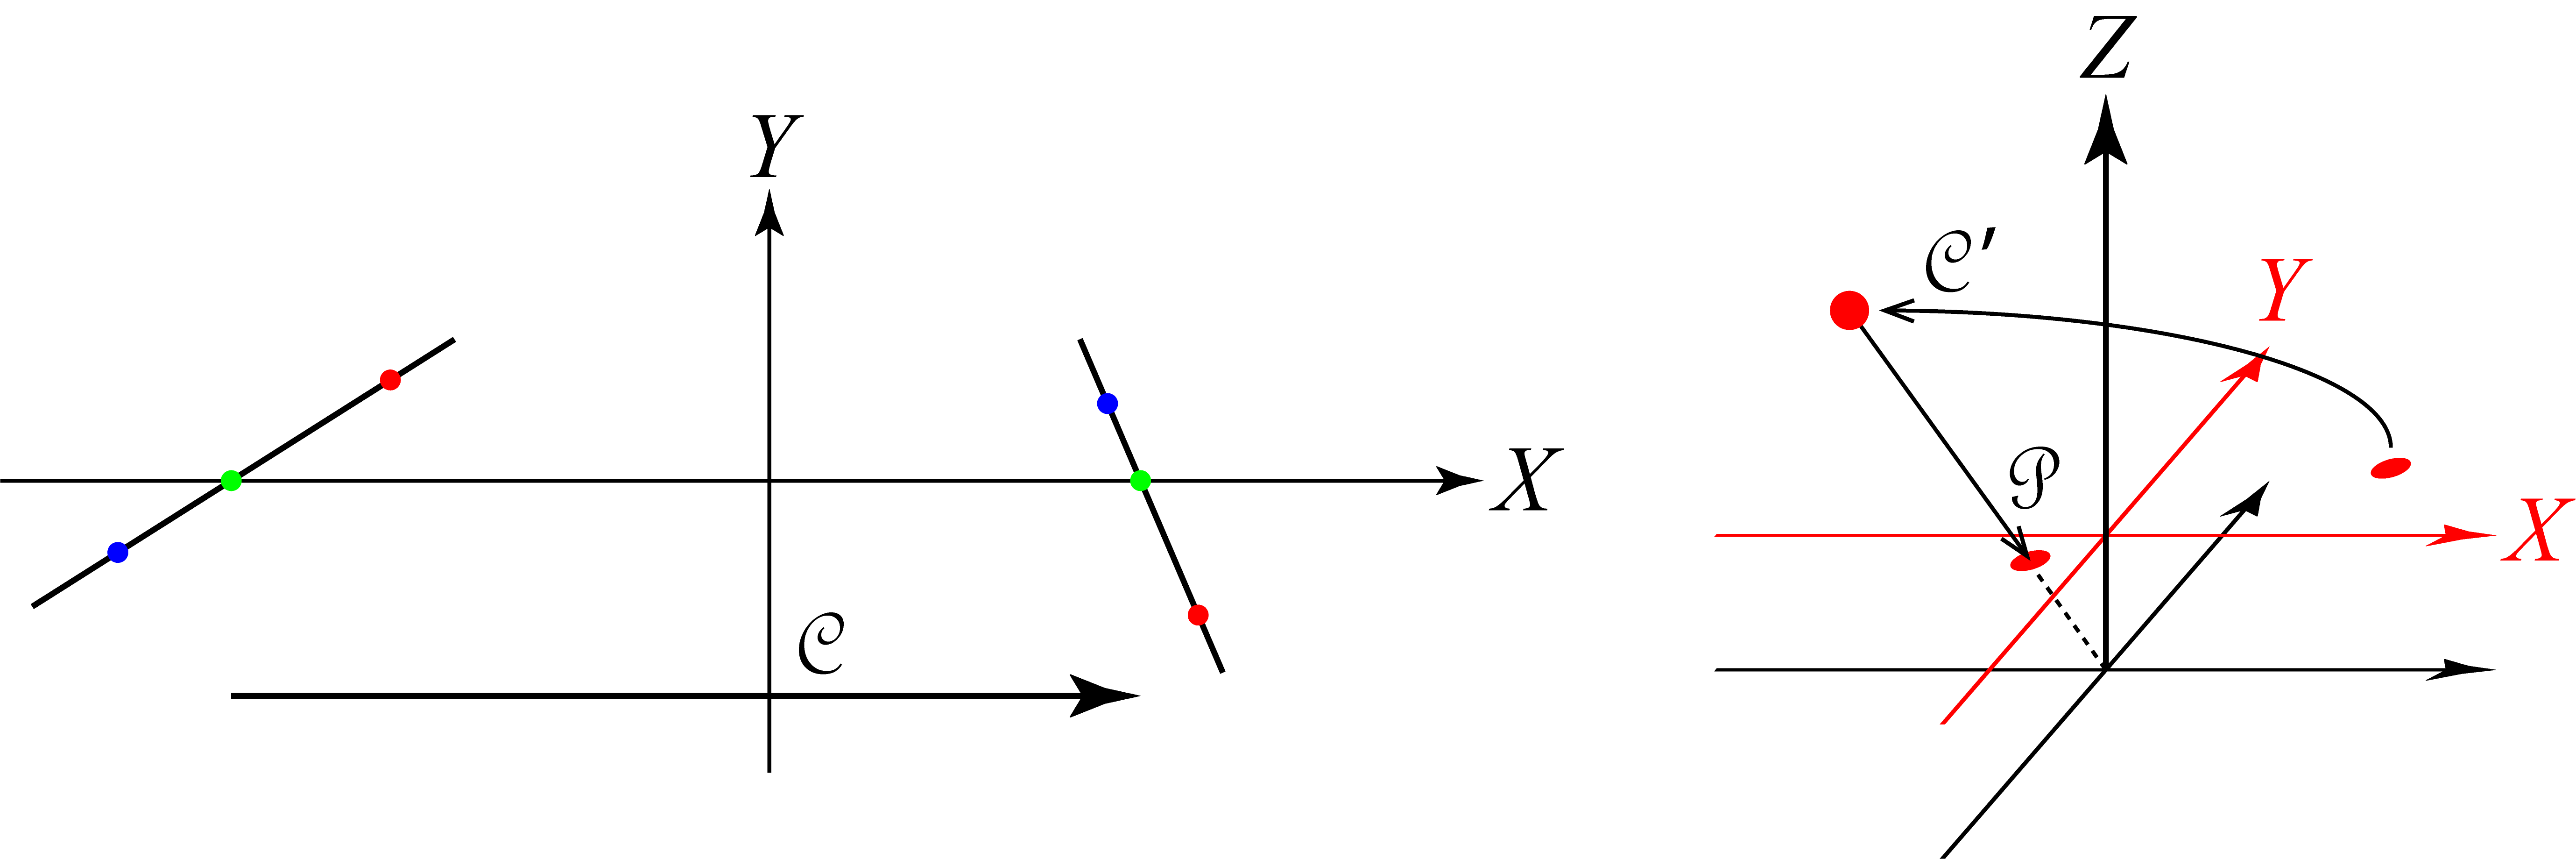
\includegraphics[width=0.7\textwidth]{image/5-7-13.png}
\caption{射影映射}
\end{figure}

那么成像作为二维平面上的点到点之间的共线性映射:
\[\mathcal{C}:\quad (X,\,Y)^{\rm T}\mapsto (X',\,Y')^{\rm T}\]

可以加一个第三维度\(Z\),\,\((X,\,Y,\,Z)\)可以以原点为中心投影到\(Z=1\)平面,\,那么原映射理解为三维内的非退化仿射变换加上投影:
\[\mathcal{P}:\quad \{(X,\,Y,\,Z)\}\mapsto(X/Z,\,Y/Z,\,1)\]
\[\mathcal{C'}:\quad \{(X,\,Y,\,1)^{\rm T}\}\mapsto \{(Z'X',\,Z'Y',\,Z')^{\rm T}\}\]
\[\begin{bmatrix} Z'X'\\Z'Y'\\Z' \end{bmatrix}=\begin{bmatrix} a&b&c\\d&e&f\\g&h&i \end{bmatrix}\begin{bmatrix} X\\Y\\1 \end{bmatrix}\quad,\quad \begin{vmatrix} a&b&c\\d&e&f\\g&h&i \end{vmatrix}\neq 0\]

此即:
\[X'=\frac{aX+bY+c}{gX+hY+i}\quad;\quad Y'=\frac{dX+eY+f}{gX+hY+i}\]

但为了使得\(Y=0\)的\(X\)轴上的点仍然被保留在\(Y'=0\)轴,\,且\(Y\)改变正负号时\(X'\)不能变,\,这给出:
\[b=h=0\quad;\quad d=f=0\]

\[X'=\frac{aX+c}{gX+i}\quad;\quad Y'=\frac{eY}{gX+i}\]

为了使变换非退化,\,要求\(e\neq 0,\,gi\neq 0,\,ac\neq 0\).

情况一是\(g=0,\,i\neq 0\),\,那么:
\[X'=\frac{a}{i}X+\frac{c}{i}\quad ;\quad Y'=\frac{e}{i}Y\]

这代表所有的望远系统,\,物像距间为线性关系,\,横向放大率在整个空间都是常数.\,两个共焦放置的薄透镜,\,平面镜与平面的折射系统在傍轴近似下都是这样的系统.\,三个放大率分别为:
\[\beta=\frac{Y'}{Y}=\frac{e}{i}\]
\[\varXi=\frac{\ud X'}{\ud X}=\frac{a}{i}\]
\[B=\left.\frac{\ud Y'}{\ud X'}\right/ \frac{\ud Y}{\ud X}=\frac{\beta}{\varXi}\quad {\rm i.e.}\quad\beta=\varXi B\]

从推导过程可以发现\(\beta=\varXi B\)其实是个恒等式.

情况二是\(g\neq 0\),\,对应所有的非望远系统.\,先考虑纵向放大率:
\[\varXi=\frac{\ud X'}{\ud X}=\frac{ai-cg}{(gX+i)^2}\]

我们指出,\,沿主光轴\(X\)方向传播的光线如果在像方仍然沿同样的\(X\)方向传播,\,那么物沿\(X\)正方向移动时必然有像也沿\(X\)正方向移动\footnote{请读者用费马原理证明它.},\,此时\(ai-cg>0\),\,这被称为\emph{折射式系统}(dioptric system).\,相反地,\,如果沿主光轴方向传播的光线如果在像方沿\(-X\)方向传播,\,此时物若沿\(X\)正方向移动,\,像将沿\(-X\)方向移动,\,被称为\emph{反射式系统}(catoptric system).\,此时我们将\(X'\)变为\(-X'\)再讨论这个问题,\,就会发现对应系数也满足\(ai-cg>0\)了.\,而更普遍的一类情况,\,物像方的主光轴甚至不会在同一个空间中重合,\,被称为\emph{折轴式系统}(off-axis system).\,此时\(X,\,X'\)本质上就位于不同空间.\,我们接下来总是默认\(ai-cg>0\)即\(\varXi>0\).

进行坐标平移:
\[x'=X'-\frac{a}{g}\quad;\quad x=-(-\frac{i}{g}-X)\]

把大写\(Y\)改为小写\(y\)便得到:
\[xx'=ff'\quad;\quad \beta=\frac{y'}{y}=-\frac{f}{x}\]
\[f=\frac{-e}{g}\quad;\quad f'=\frac{ai-cg}{(-e)g}\]

这便是牛顿式的成像公式.\,我们从中可以发现:
\[\frac{f'}{f}=\frac{ai-cg}{e^2}>0\]

可见两个焦距一定同号.\,它与折射率的关系是我们接下来要解决的关键问题.






%\section{非傍轴成像}